\documentclass{thesis}
\usepackage{thesis}
\usepackage{parskip}
\usepackage{hepnames}
\usepackage[printonlyused]{acronym}
\usepackage{ptdr-definitions}
\usepackage{slashed}
\usepackage{multirow}
\usepackage{amssymb}
\usepackage{import}
\usepackage{colortbl}
\usepackage{hhline}

%% You can set the line spacing this way
%\setallspacing{double}
%% or a section at a time like this
%\setfrontmatterspacing{double}


%% Define a few useful shorthands
\newcommand{\emu}{\Pe\Pgm}
\newcommand{\ee}{\Pe\Pe}
\newcommand{\mumu}{\Pgm\Pgm}
\newcommand{\mutau}{\Pgm\Pgth}
\newcommand{\etau}{\Pe\Pgth}
\newcommand{\tautau}{\Pgth\Pgth}

\newcommand{\WJets}{\ensuremath{\PW}{+}\text{jets}\xspace}
\newcommand{\mhmax}{\ensuremath{m_{\Ph}^{\text{max}}}\xspace}
\newcommand{\ttbar}{\ensuremath{\Pqt\Paqt}\xspace}
\newcommand{\ZToTauTau}{\ensuremath{\PZ\to\Pgt\Pgt}\xspace}
\newcommand{\HToTauTau}{\ensuremath{\PH\to\Pgt\Pgt}\xspace}

\renewcommand{\listfigurename}{List of figures}
\renewcommand{\listtablename}{List of tables}



%% PDF metadata
\makeatletter
\@ifpackageloaded{hyperref}{%
\hypersetup{%
pdftitle = {Searches for invisibly decaying Higgs bosons with the CMS detector},
pdfsubject = {Patrick Dunne's PhD thesis},
pdfkeywords = {CMS, H, physics, LHC, Higgs},
pdfauthor = {\textcopyright\ Patrick Dunne},
linkcolor=black
}
}{}
\makeatother

%% Define the thesis title and author
\title{Searches for invisibly decaying Higgs bosons with the CMS detector}
\author{Patrick James Dunne}

%% Start the document
\begin{document}

%% Define the un-numbered front matter (cover pages, rubrik and table of contents)
\begin{frontmatter}
  %% Title
%??UPDATE THIS
\titlepage[of Imperial College London]%
{A dissertation submitted to Imperial College London\\
  for the degree of Doctor of Philosophy}

\newpage
The copyright of this thesis rests with the author and is made available under a Creative Commons
Attribution Non-Commercial No Derivatives licence. Researchers are free to copy, distribute or
transmit the thesis on the condition that they attribute it, that they do not use it for commercial
purposes and that they do not alter, transform or build upon it. For any reuse or redistribution,
researchers must make clear to others the licence terms of this work

%% Abstract
\begin{abstract}%[\smaller \thetitle\\ \vspace*{1cm} \smaller {\theauthor}]
  %\thispagestyle{empty}
  Searches for invisibly decaying Higgs bosons using the Compact Muon Solenoid (CMS) detector at the CERN Large Hadron Collider (LHC) and their interpretations are described. These searches are motivated both by a desire to characterise the newly observed Higgs boson, and by the cosmological observation of very weakly interacting matter in the universe, which is called dark matter. In order to provide context for these searches, introductions to the Standard Model (SM) of particle physics and several extensions to the SM which incorporate dark matter are given.

The searches described in this thesis use data recorded in proton-proton collisions in 2012 and focus on the most sensitive mode, Vector Boson Fusion (VBF) production. The first search uses 19.5 \invfb\, of data promptly reconstructed in 2012 and results in an observed (expected) limit on the invisible branching fraction of the 125 \GeV Higgs boson, \BRinv, of 0.65 (0.49) at the 95\% confidence level (CL)~\cite{Chatrchyan:2014tja}. The second search uses 19.2 \invfb\,of data collected using triggers with looser thresholds and reconstructed later, in 2013. This search resulted in an observed (expected) limit on \BRinv of 0.57 (0.40) at the 95\% CL~\cite{CMS-PAS-HIG-14-038}.

Combinations of these searches with searches in other production channels are also described, the most sensitive of which results in an observed (expected) limit on \BRinv of 0.36 (0.30) at 95\% CL~\cite{CMS-PAS-HIG-15-012}. Projections of the sensitivity of these analyses in Run 2 and interpretations of their results as limits on various models of dark matter are also given~\cite{ourdmpaper}.
\end{abstract}


%% Declaration
\begin{declaration}
  This dissertation is the result of my own work. Where figures and results are taken from other sources this is indicated by an appropriate reference. Some figures referenced as from other sources were created by me, but appear in other public documents. 

The description of the analysis described in \ChapterRef{chap:prompt} follows \ReferenceRef{ARTICLE:CMSAN-12-403}, which includes elements of my work, and was made public in \ReferenceRef{Chatrchyan:2014tja}.. Specifically, I was responsible for cross-checking the results of all the $\PW+$jets background estimations, I contributed to the development of the formula used to carry out the $\PZ+$jets background estimation, I calculated and cross-checked several of the systematic uncertainties, I produced plots of the discriminating variables for final publication, and I performed all limit setting and production of limit plots. 

I was the main analyser for the analysis described in \ChapterRef{chap:parked}, responsible for all steps of the analysis including trigger efficiency measurement, background estimation, systematic uncertainty studies and limit setting. The QCD background estimation method was developed and implemented collaboratively with other members of the Imperial College high energy physics (HEP) group. This work was made public in \ReferenceRef{CMS-PAS-HIG-14-038}.

I was also solely responsible for the combinations described in \ChapterRef{chap:comb}. For the interpretations of the VBF invisibly decaying Higgs boson searches as limits on dark mater models described in \ChapterRef{chap:interp} I worked collaboratively with theorists at Rutgers University and members of the Imperial College and Bristol University HEP groups. This work was made public in \ReferenceRef{ourdmpaper}.

As well as the work described in this thesis I have also carried out preparations for a search for VBF produced invisibly decaying Higgs bosons using Run 2 data from the LHC. These preparations have included measurements of the trigger efficiency for the triggers used in 2015 CMS data taking and comparisons of the kinematic distributions of signal and background events at the increased 13 TeV centre of mass energy used in Run 2 with those from Run 1, this work is currently under approval. Together with a new PhD student, I have also carried out a combination of the first Run 2 invisibly decaying Higgs boson searches in the VBF and ZH channels with those in Run 1, which is currently being approved for publication.


  \vspace*{1cm}
  \begin{flushright}
    Patrick James Dunne
  \end{flushright}
\end{declaration}


%% Acknowledgements
\begin{acknowledgements}
%??Stephanie, Mum, Dad rest of family
%??Gavin, Dave, Anne Marie, Joao, Jim, Andrew, Nick all other colleagues
%??STFC, and IC
\end{acknowledgements}


%% Preface
%\begin{preface}
%\end{preface}

%% ToC
\tableofcontents

%% Strictly optional!
%\frontquote%
%{Writing in English is the most ingenious torture\\
%   ever devised for sins committed in previous lives.}%
%  {James Joyce}

\end{frontmatter}

%% Start the content body of the thesis
\begin{mainmatter}
  %% Actually, more semantic chapter filenames are better, like "chap-bgtheory.tex"
  \import{}{theory}
  \import{}{detector}
  \import{}{obj}
  \import{}{prompt}
  \import{}{parked}
  \import{}{comb}
  \import{}{interp}
  %\import{}{run2} %??relegated to declaration

  %% To ignore a specific chapter while working on another,
  %% making the build faster, comment it out like this:
  %\input{chap4}
\end{mainmatter}

%% Produce the appendices
\begin{appendices}
  \chapter{Parked data trigger efficiencies}
\label{app:trigeffs}
This appendix contains the trigger efficiency curves with overlaid error function fits and there errors as described in \SectionRef{sec:parkedtrigger}. Due to the event selection applied in the parked data analysis only the highest bin in \Mjj is used.

\begin{figure}[h!]
  \begin{center}
    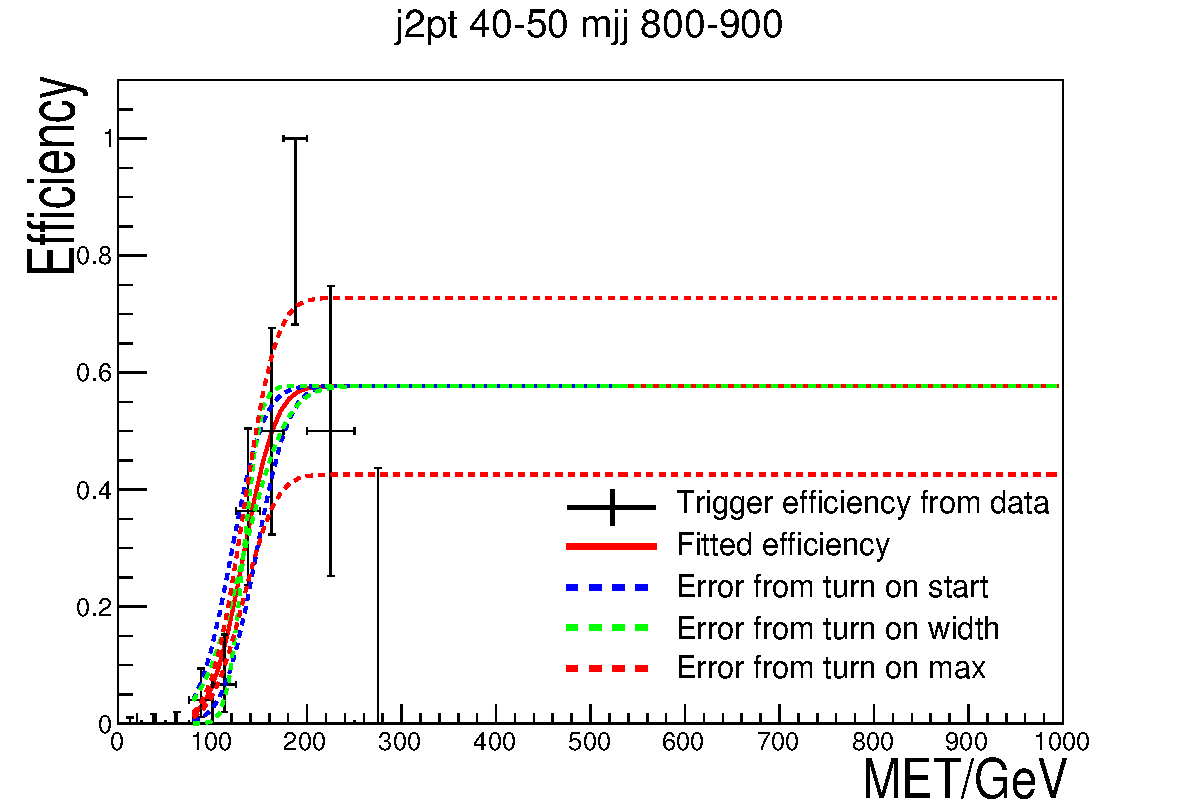
\includegraphics[width=.6\largefigwidth]{plots/parked/trigfitplots/hData_MET_1D_23A.pdf}
    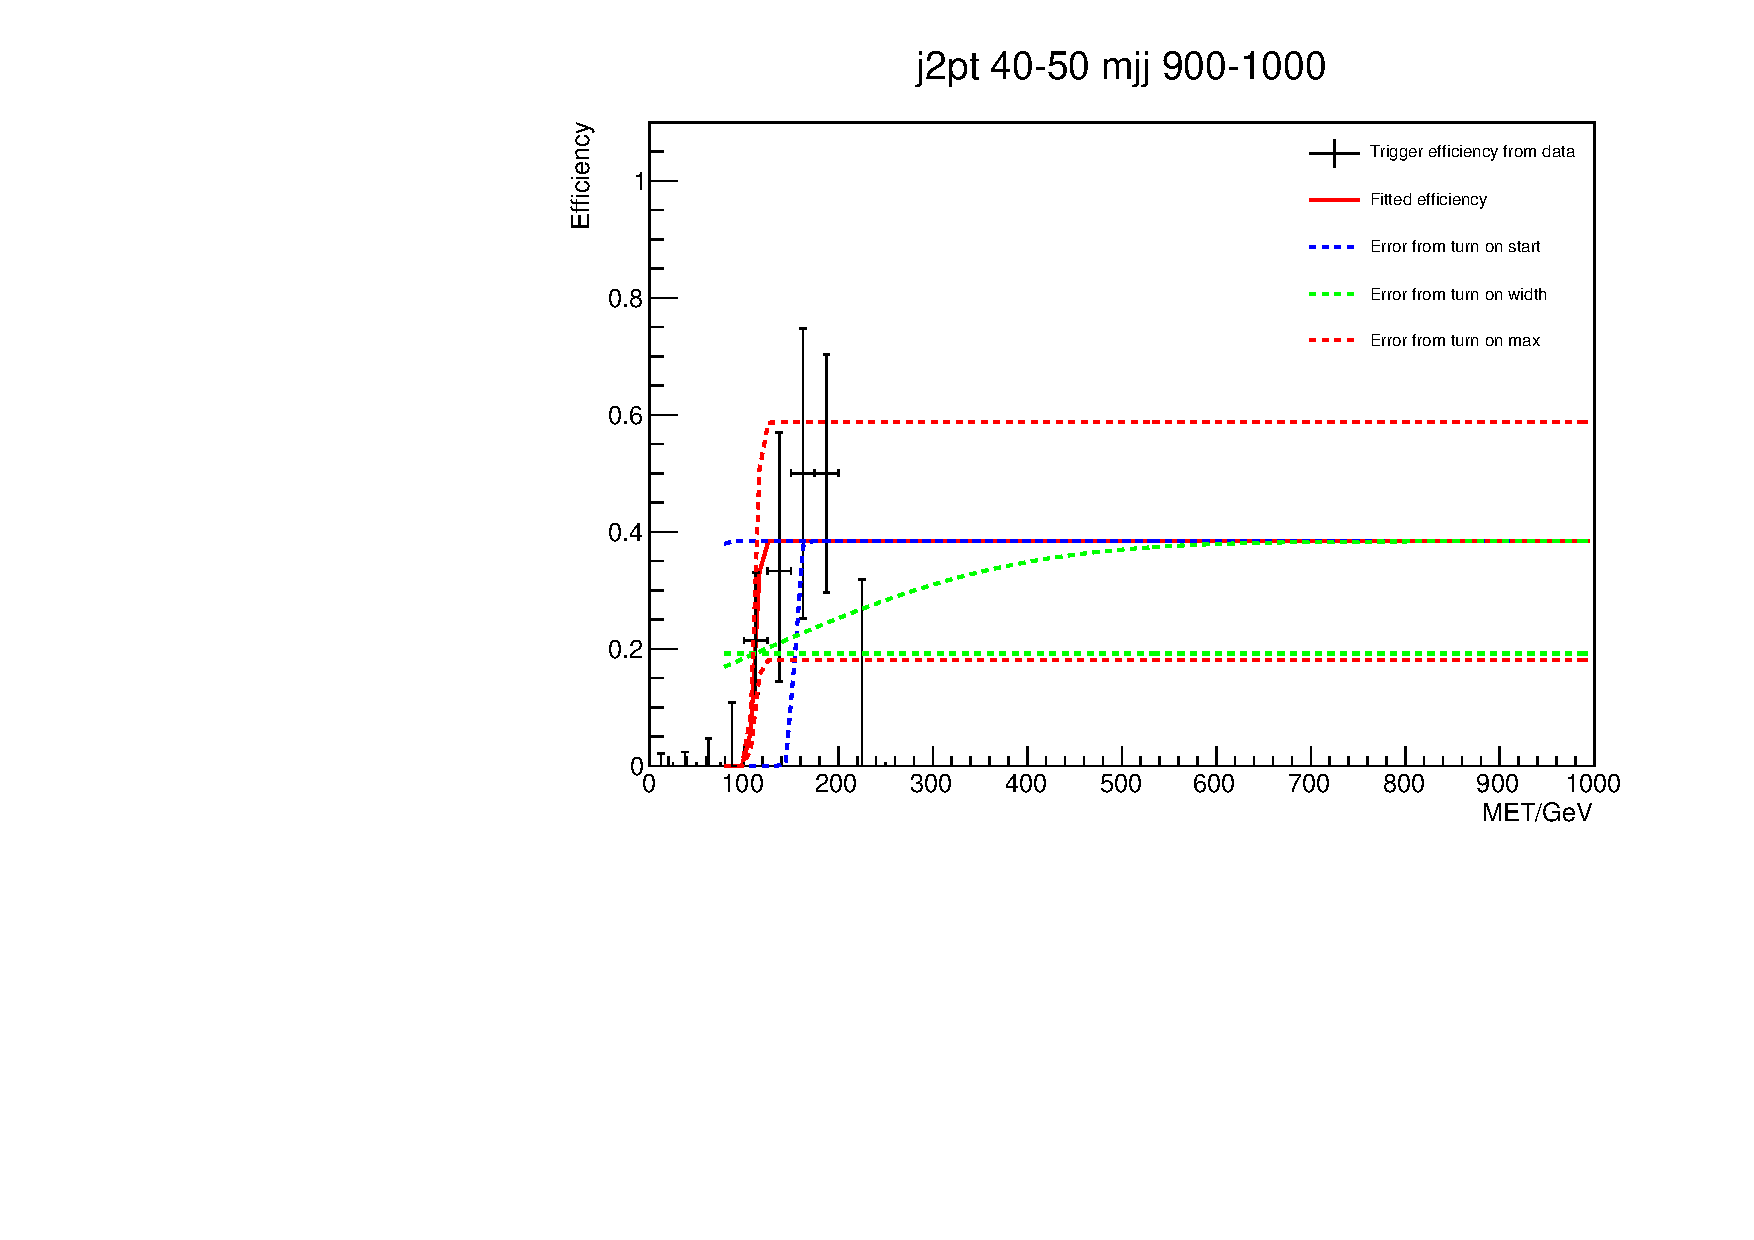
\includegraphics[width=.6\largefigwidth]{plots/parked/trigfitplots/hData_MET_1D_24A.pdf}

    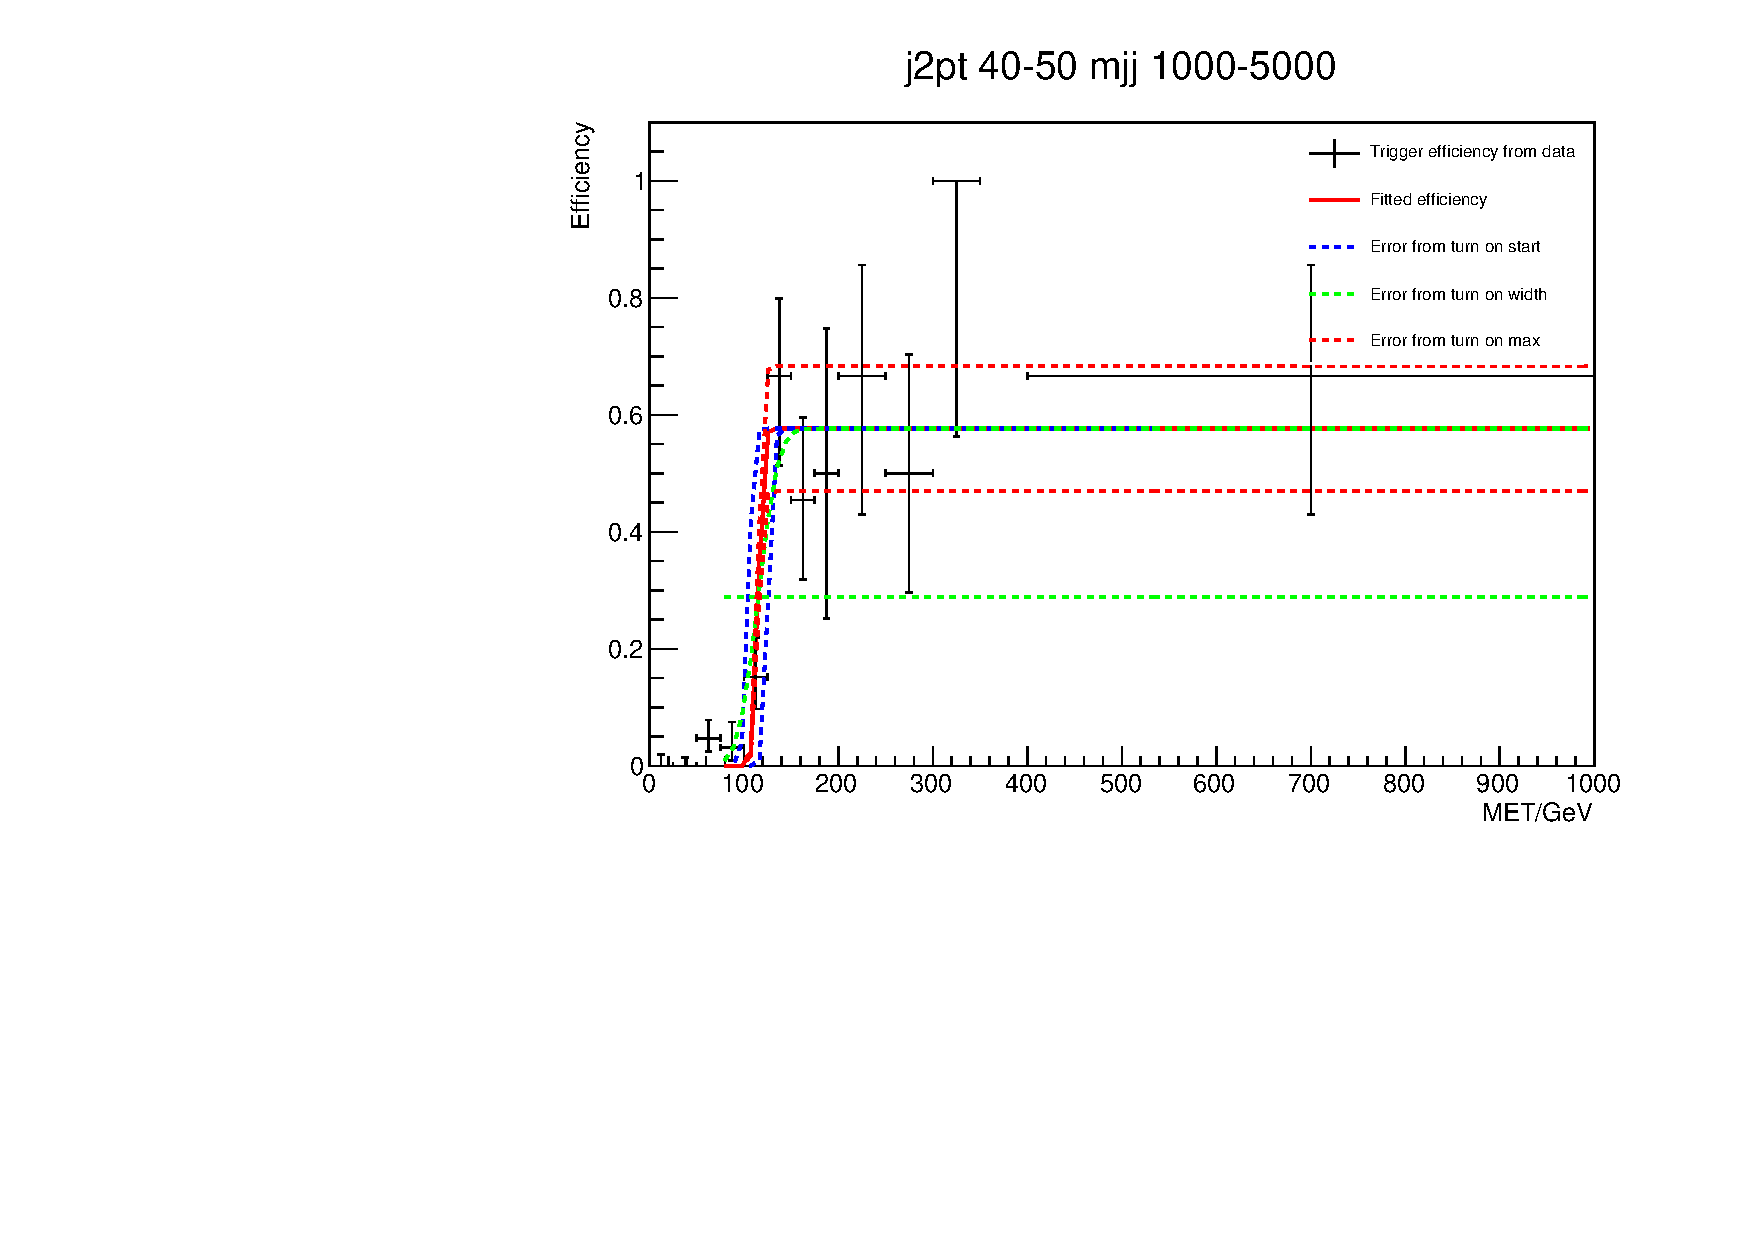
\includegraphics[width=.6\largefigwidth]{plots/parked/trigfitplots/hData_MET_1D_25A.pdf}
    \caption{The measured efficiency of the trigger used in run A as a function of MET in bins of dijet mass (mjj) and sub-leading jet $p_{T}$ (j2pt). The bin that each plot corresponds to is displayed at the top of the plot}
    \label{fig:trigfitplotsA1}
  \end{center}
\end{figure}

\begin{figure}[h!]
  \begin{center}
    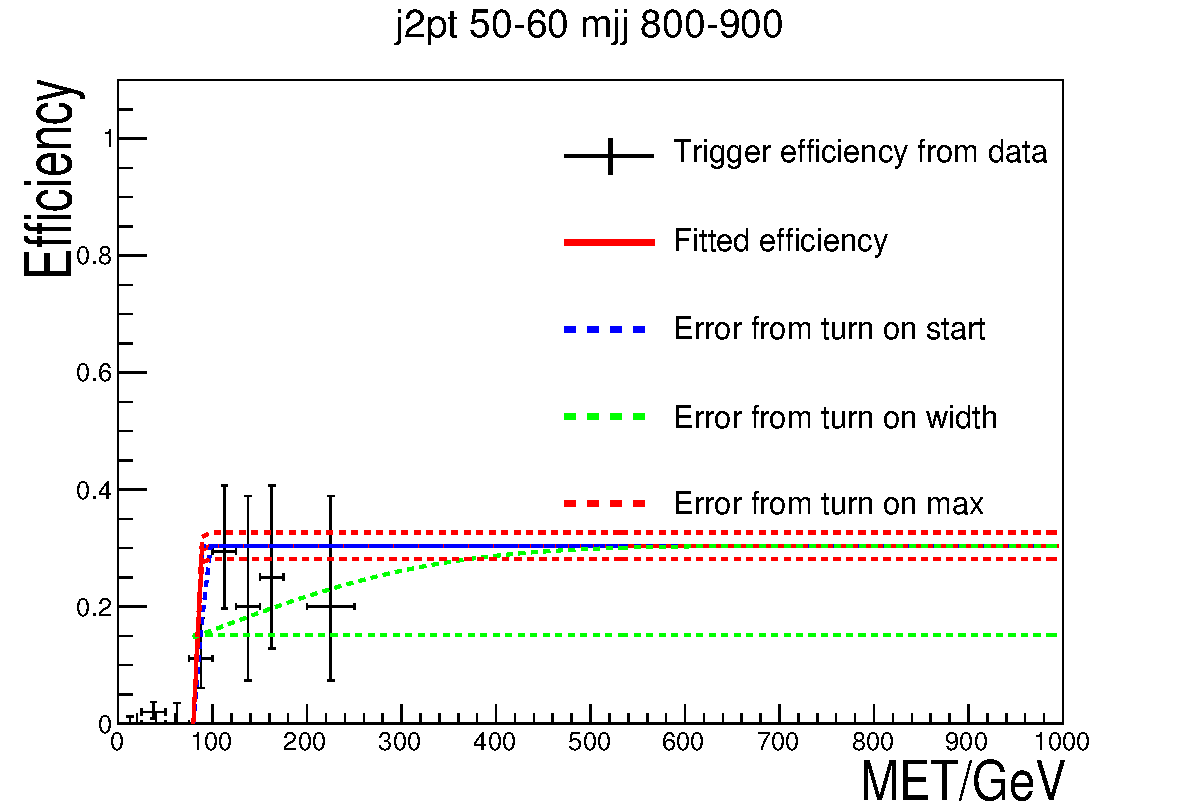
\includegraphics[width=.6\largefigwidth]{plots/parked/trigfitplots/hData_MET_1D_33A.pdf}
    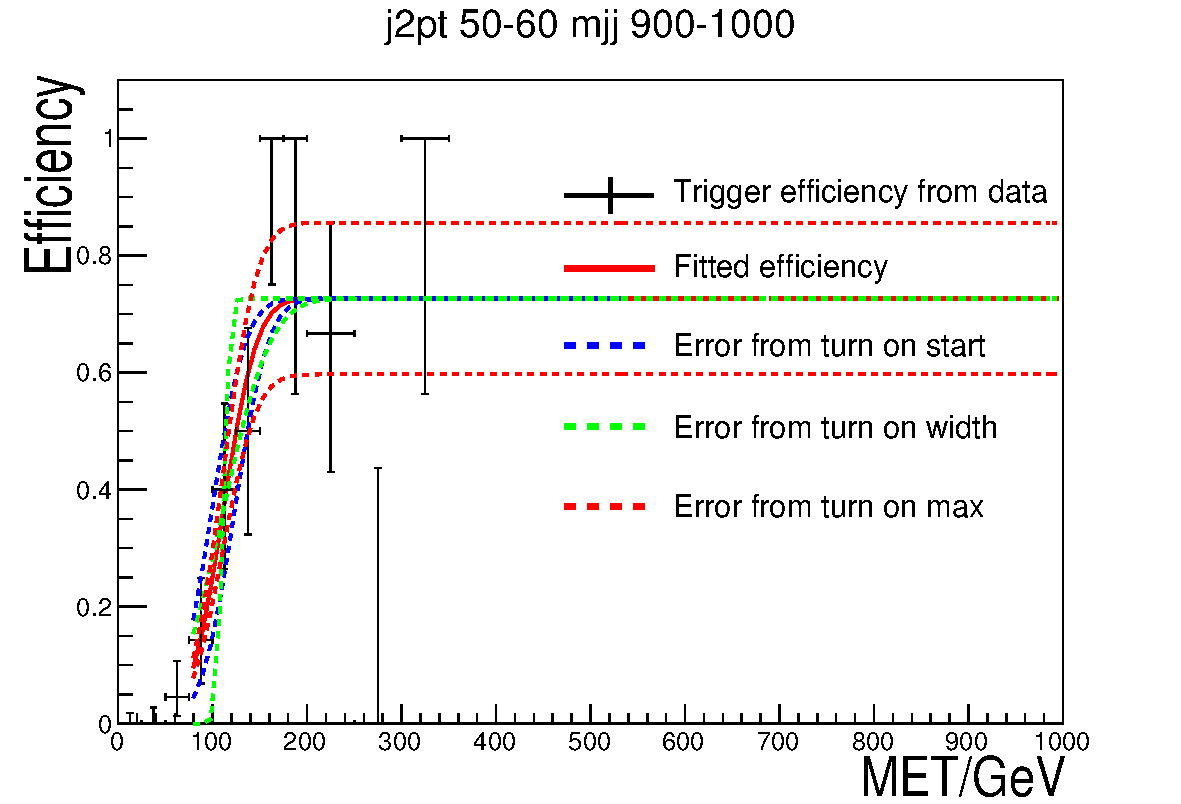
\includegraphics[width=.6\largefigwidth]{plots/parked/trigfitplots/hData_MET_1D_34A.pdf}

    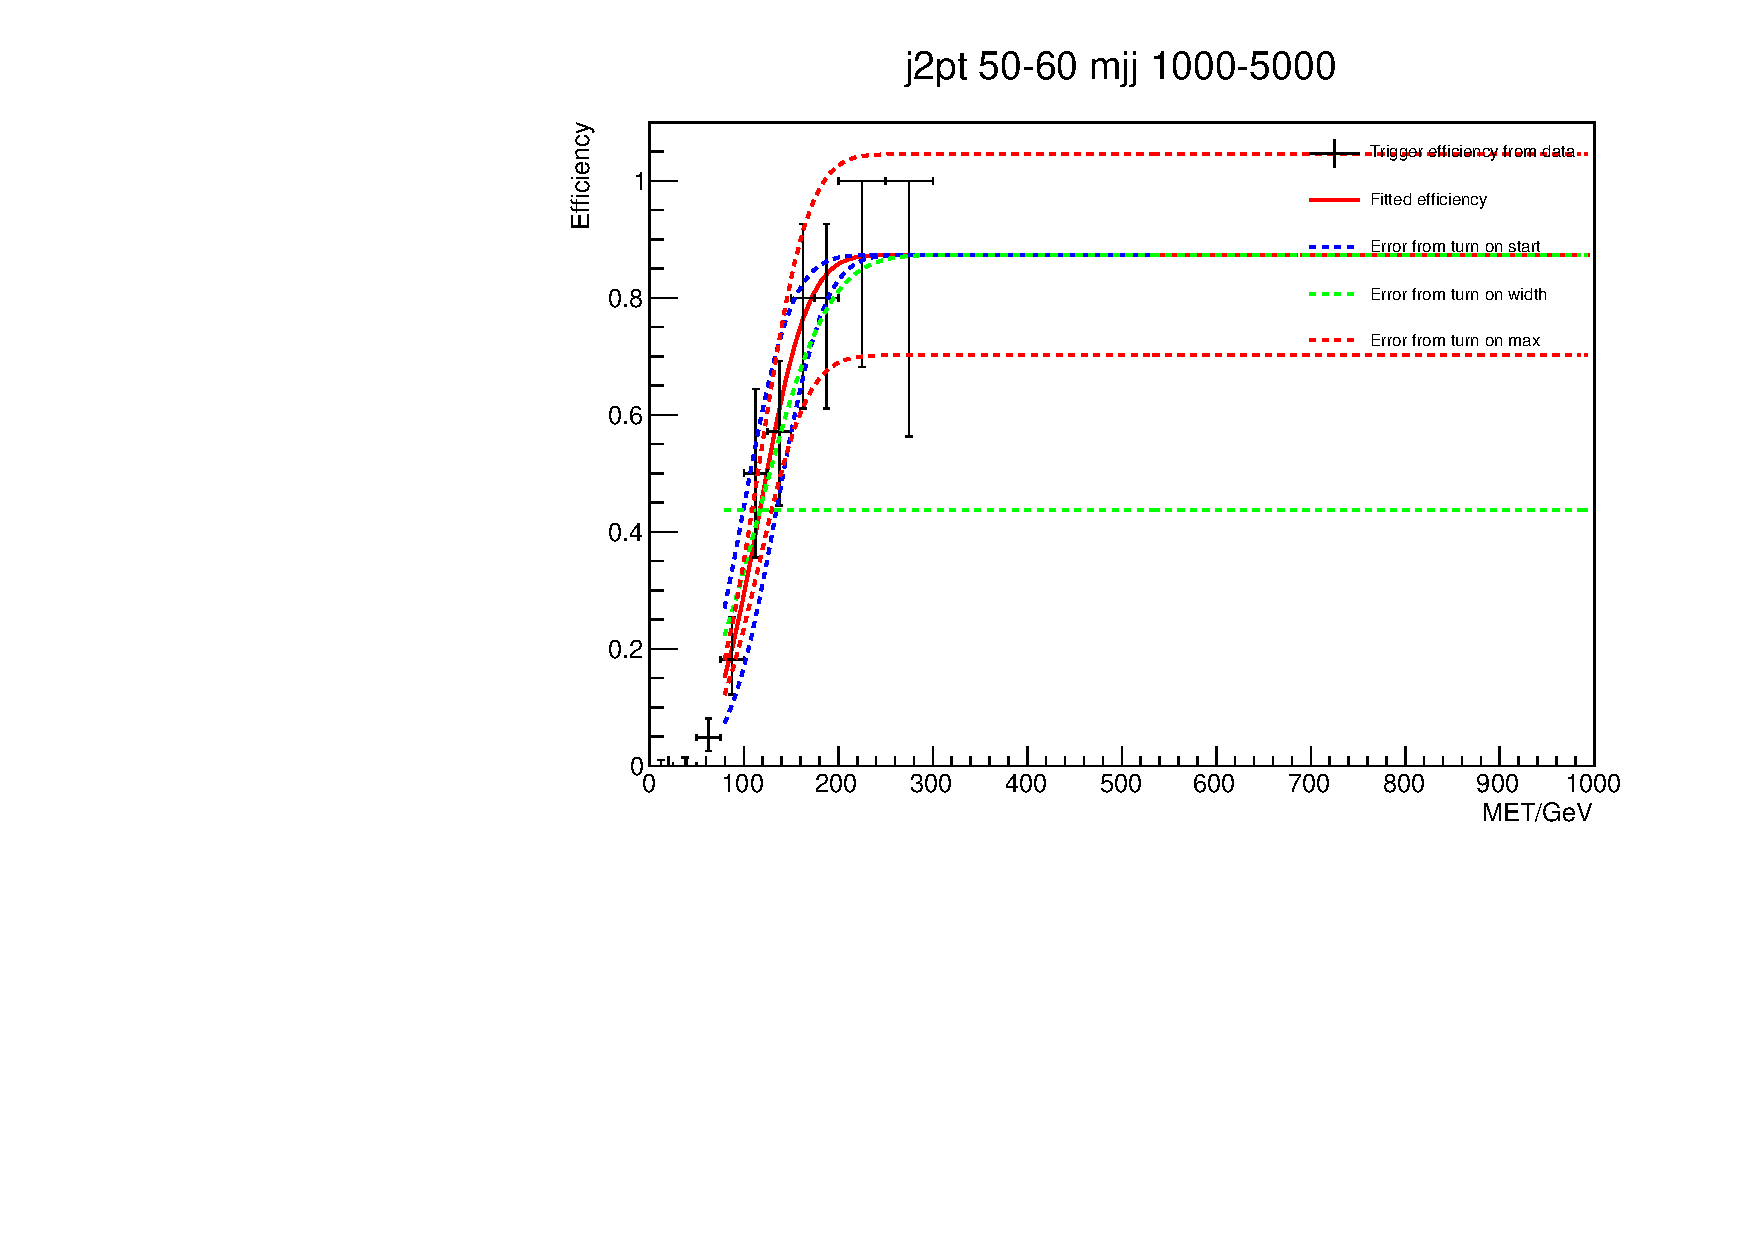
\includegraphics[width=.6\largefigwidth]{plots/parked/trigfitplots/hData_MET_1D_35A.pdf}
    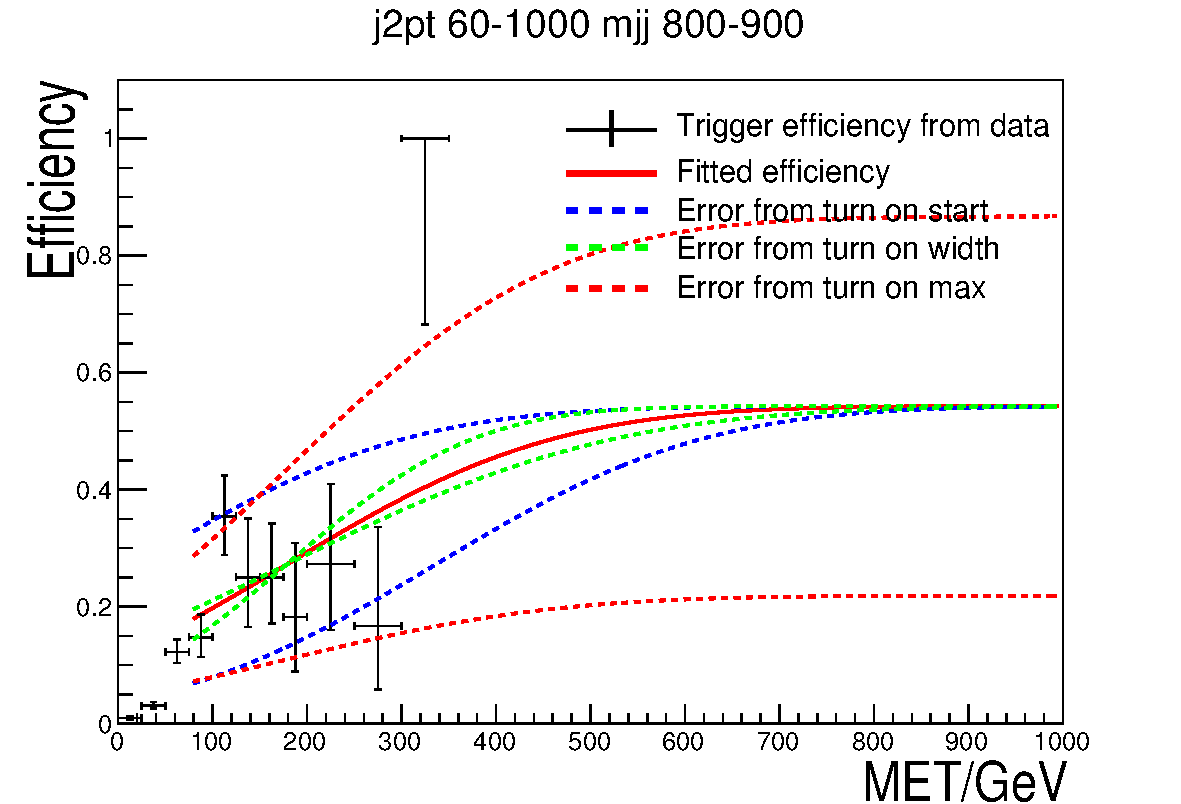
\includegraphics[width=.6\largefigwidth]{plots/parked/trigfitplots/hData_MET_1D_43A.pdf}

    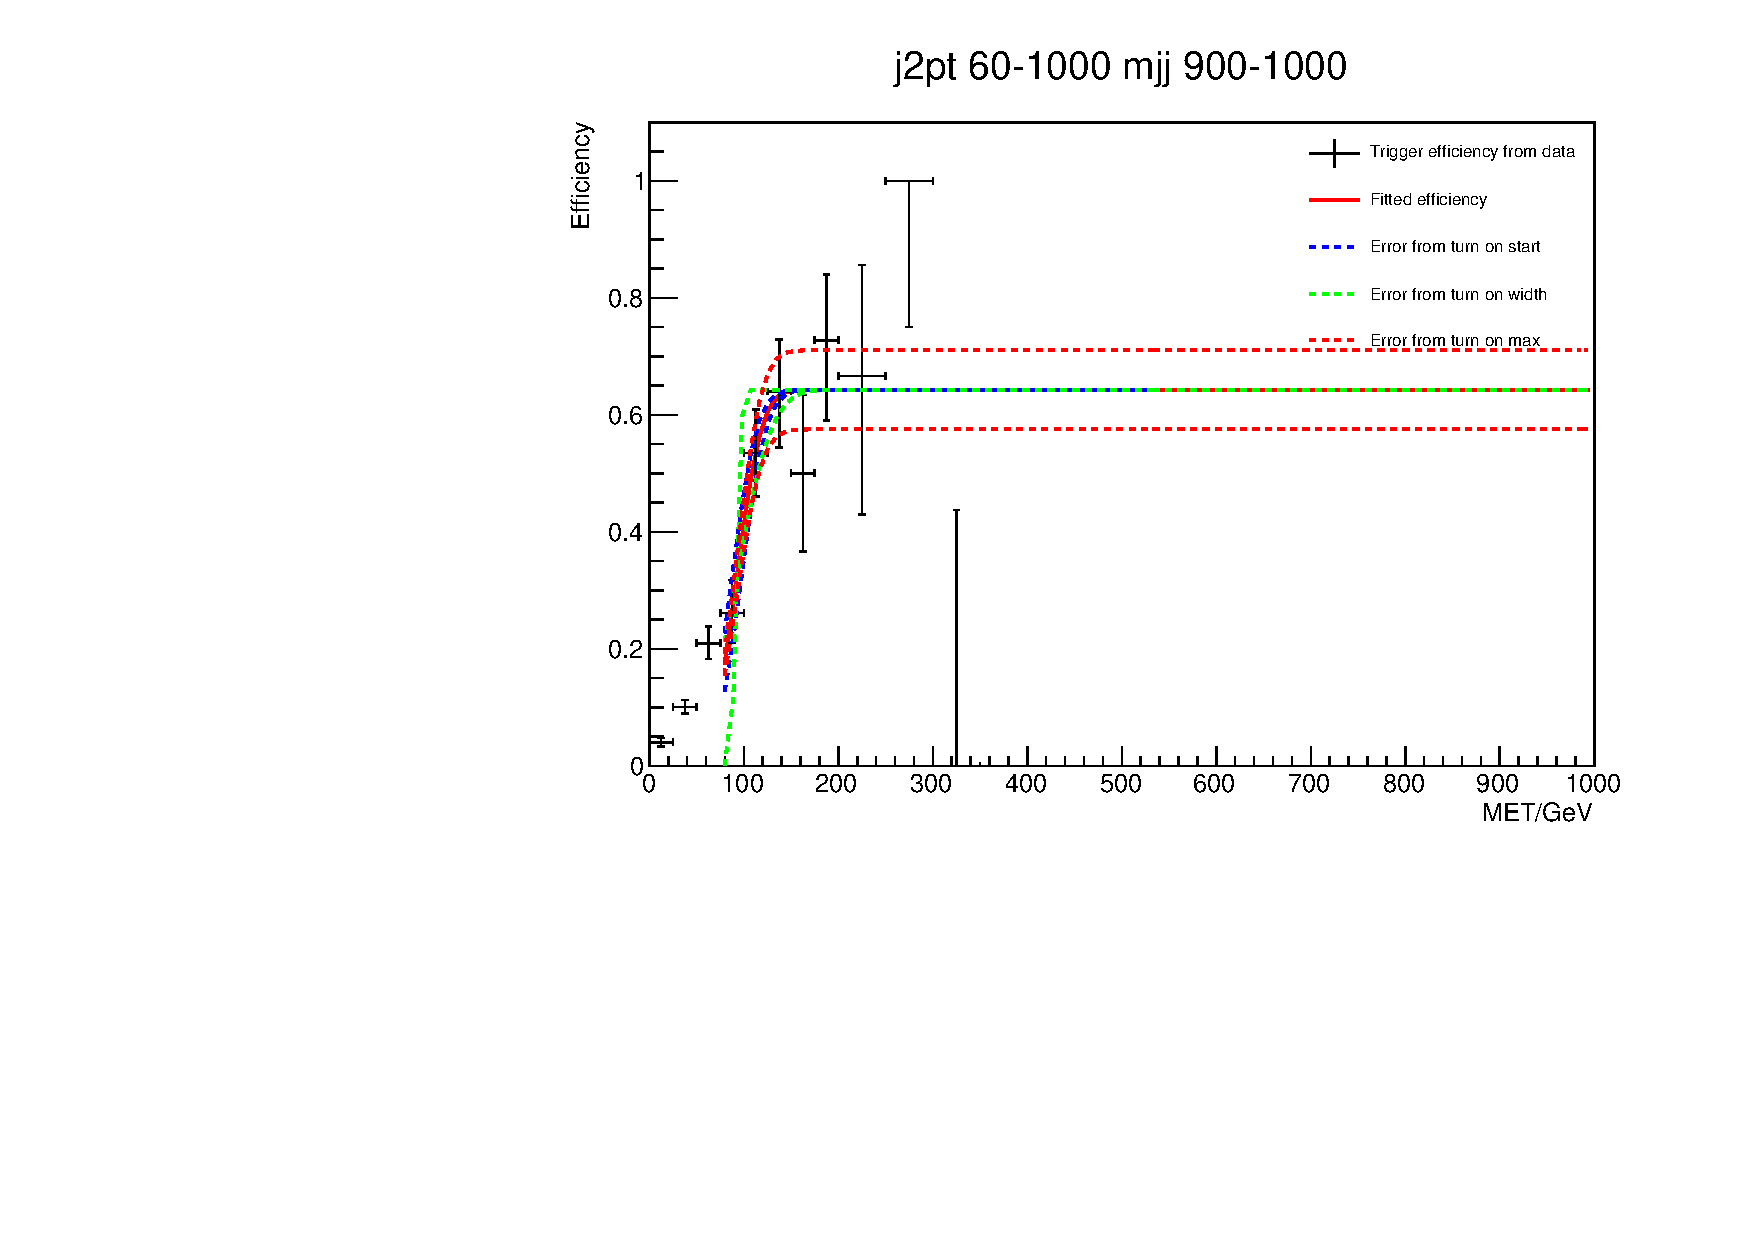
\includegraphics[width=.6\largefigwidth]{plots/parked/trigfitplots/hData_MET_1D_44A.pdf}
    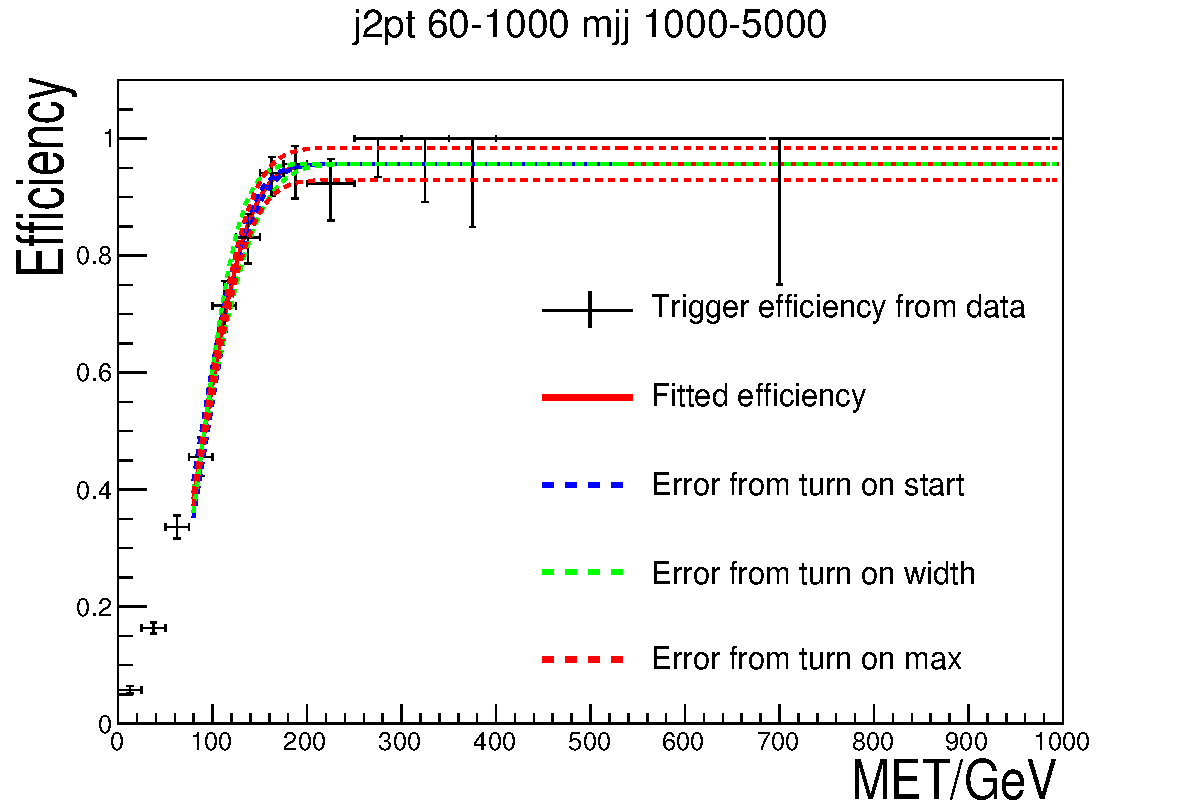
\includegraphics[width=.6\largefigwidth]{plots/parked/trigfitplots/hData_MET_1D_45A.pdf}
    \caption{The measured efficiency of the trigger used in run A as a function of MET in bins of dijet mass (mjj) and sub-leading jet $p_{T}$ (j2pt). The bin that each plot corresponds to is displayed at the top of the plot}
    \label{fig:trigfitplotsA2}
  \end{center}
\end{figure}

\begin{figure}[h!]
  \begin{center}
    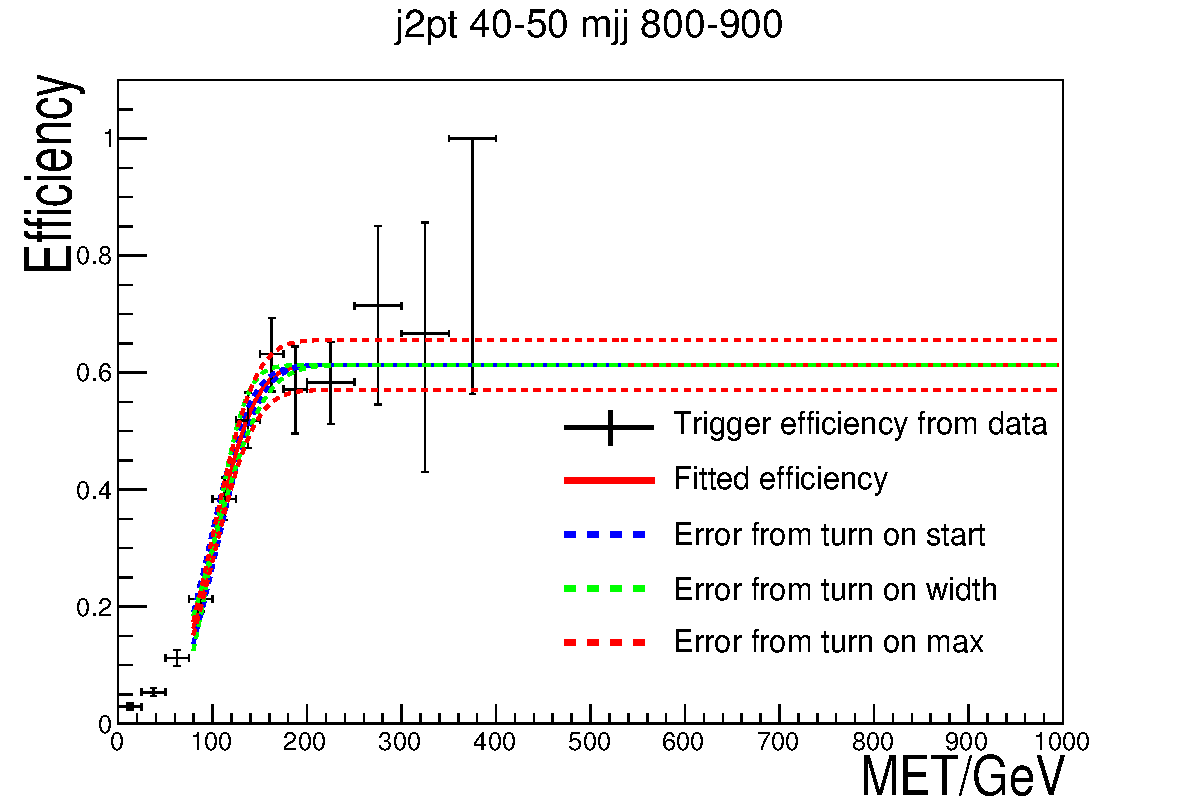
\includegraphics[width=.6\largefigwidth]{plots/parked/trigfitplots/hData_MET_1D_23BC.pdf}
    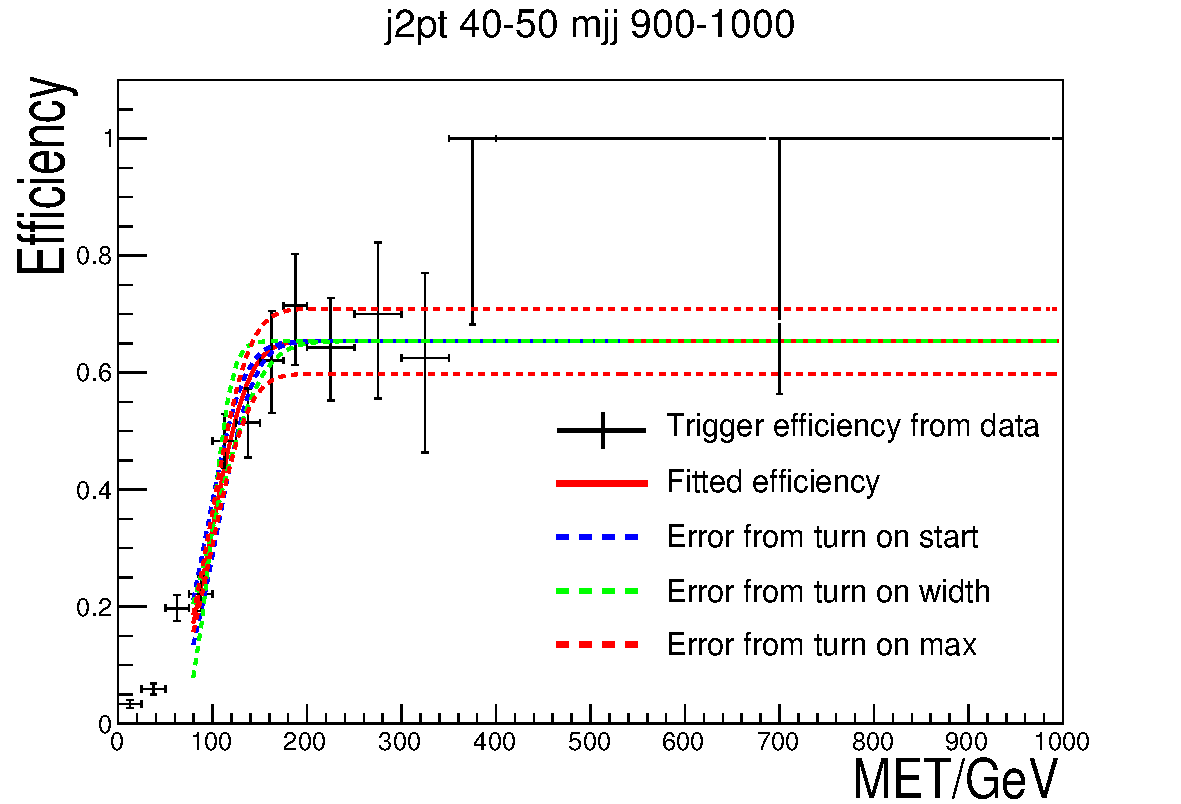
\includegraphics[width=.6\largefigwidth]{plots/parked/trigfitplots/hData_MET_1D_24BC.pdf}

    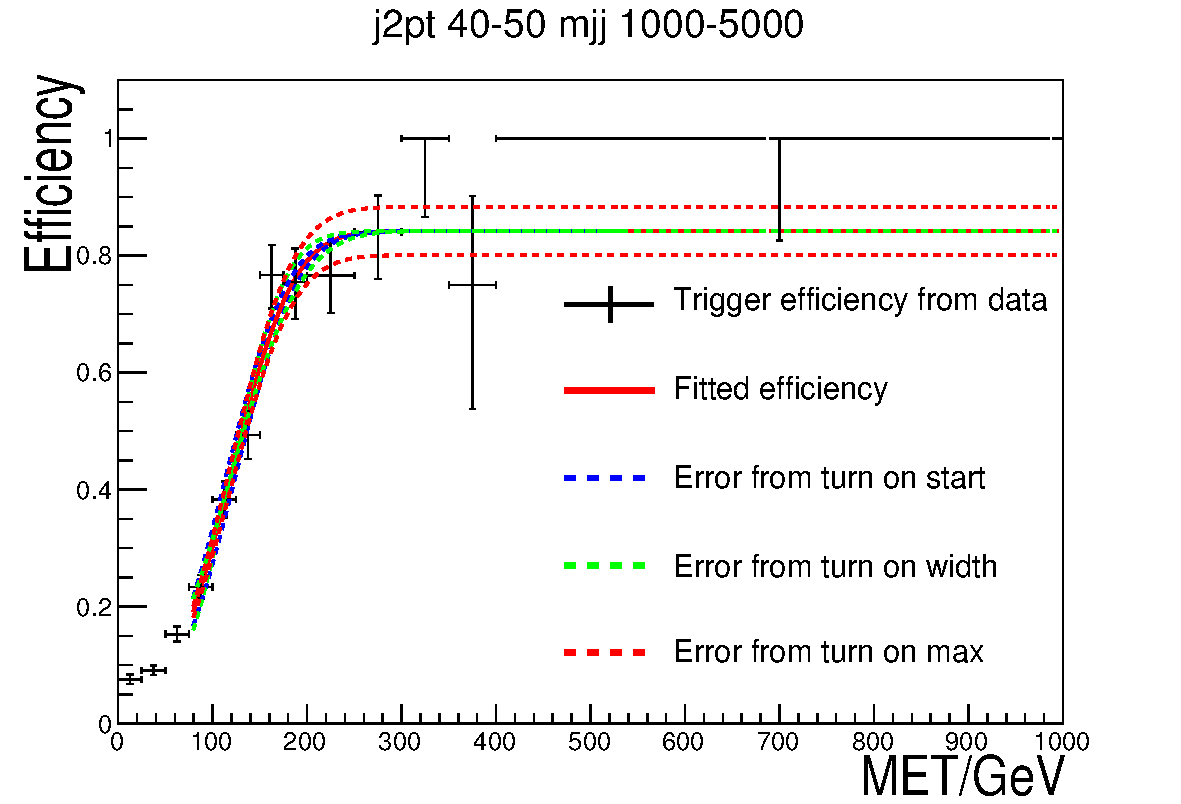
\includegraphics[width=.6\largefigwidth]{plots/parked/trigfitplots/hData_MET_1D_25BC.pdf}
    \caption{The measured efficiency of the trigger used in runs B and C as a function of MET in bins of dijet mass (mjj) and sub-leading jet $p_{T}$ (j2pt). The bin that each plot corresponds to is displayed at the top of the plot}
    \label{fig:trigfitplotsBC1}
  \end{center}
\end{figure}

\begin{figure}
  \begin{center}
    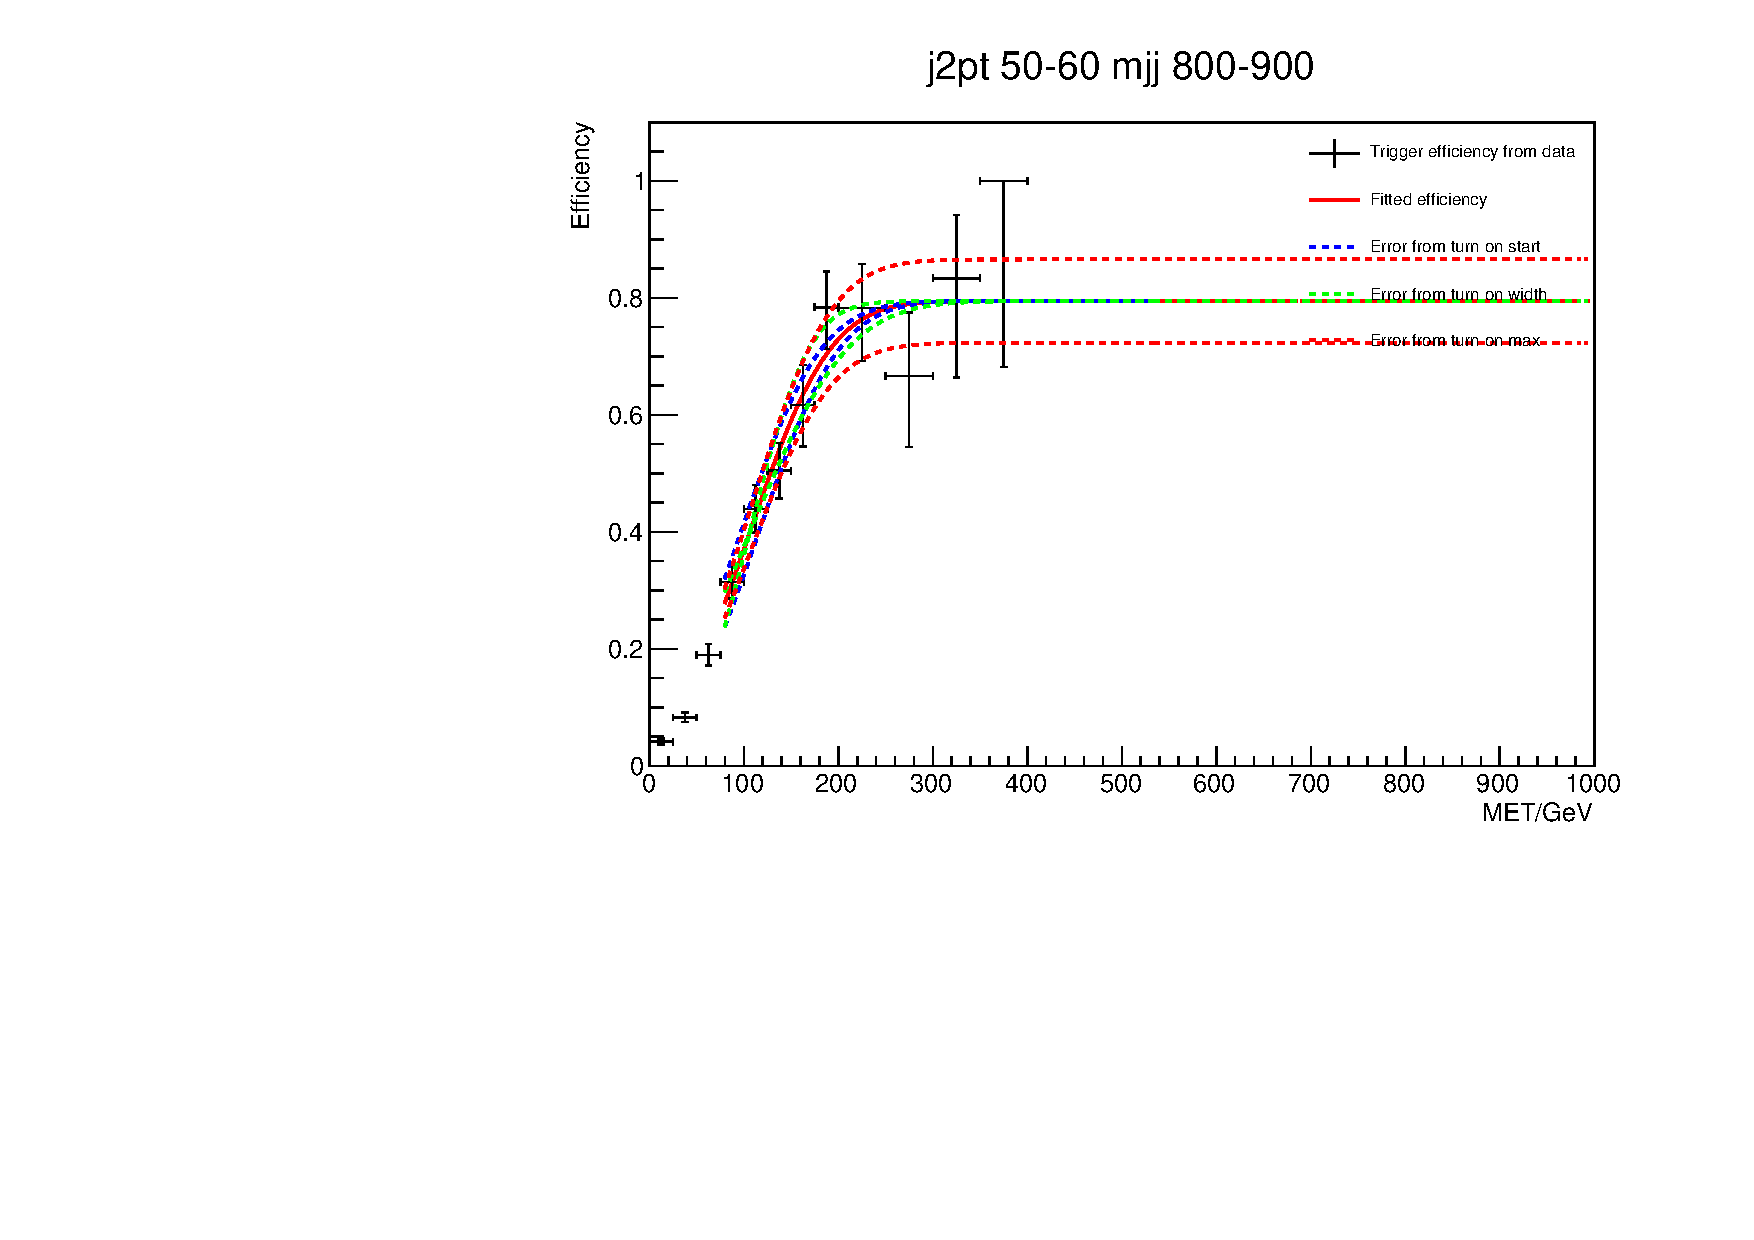
\includegraphics[width=.6\largefigwidth]{plots/parked/trigfitplots/hData_MET_1D_33BC.pdf}
    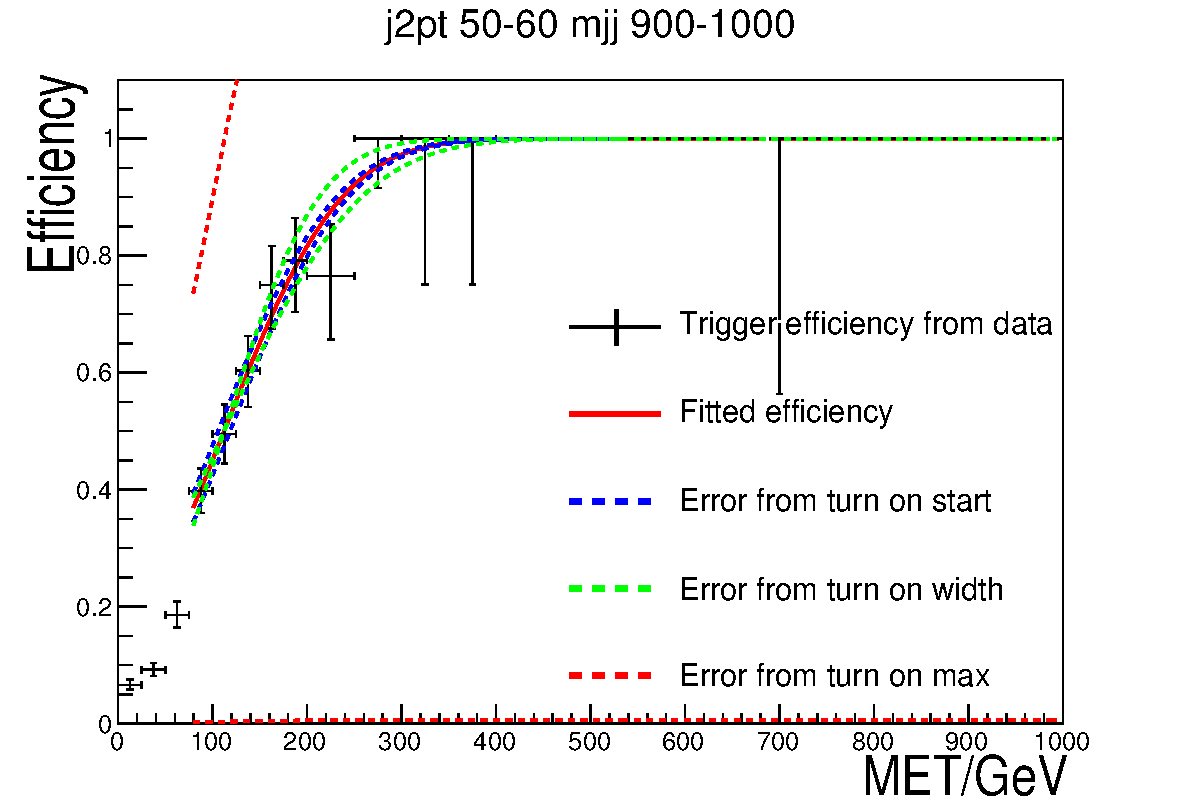
\includegraphics[width=.6\largefigwidth]{plots/parked/trigfitplots/hData_MET_1D_34BC.pdf}

    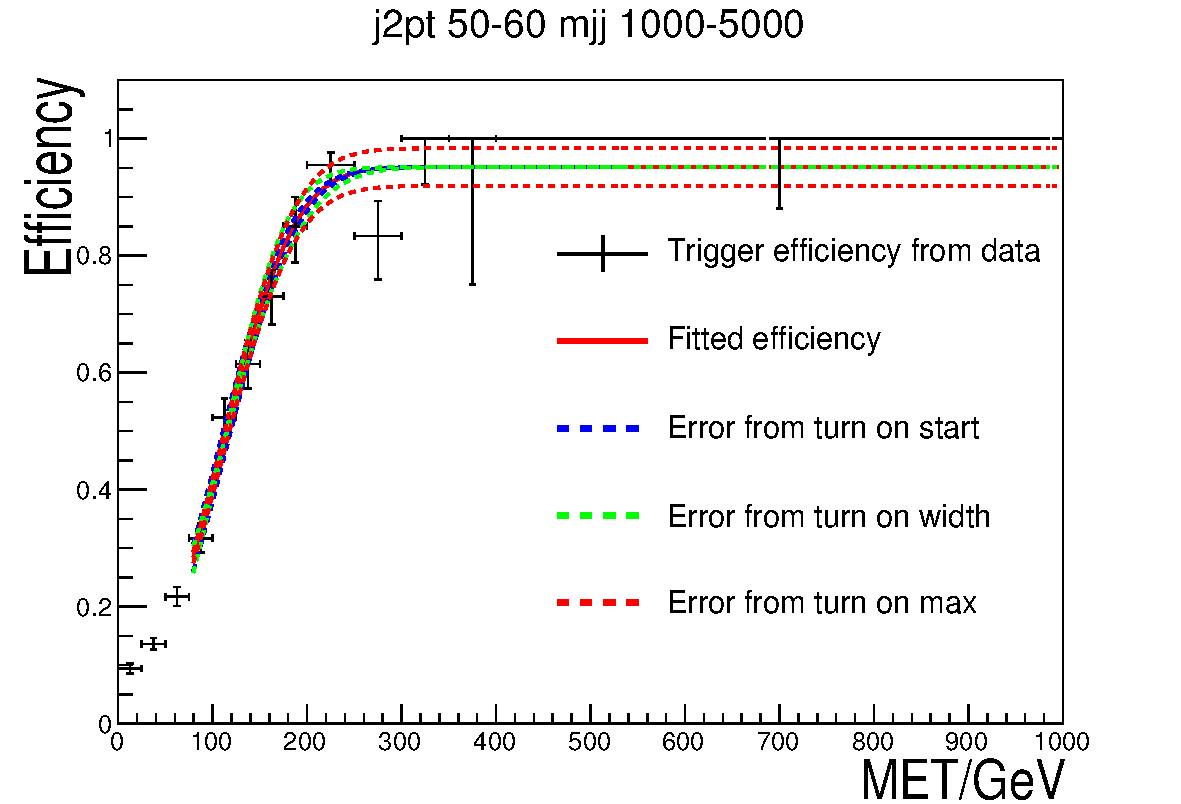
\includegraphics[width=.6\largefigwidth]{plots/parked/trigfitplots/hData_MET_1D_35BC.pdf}
    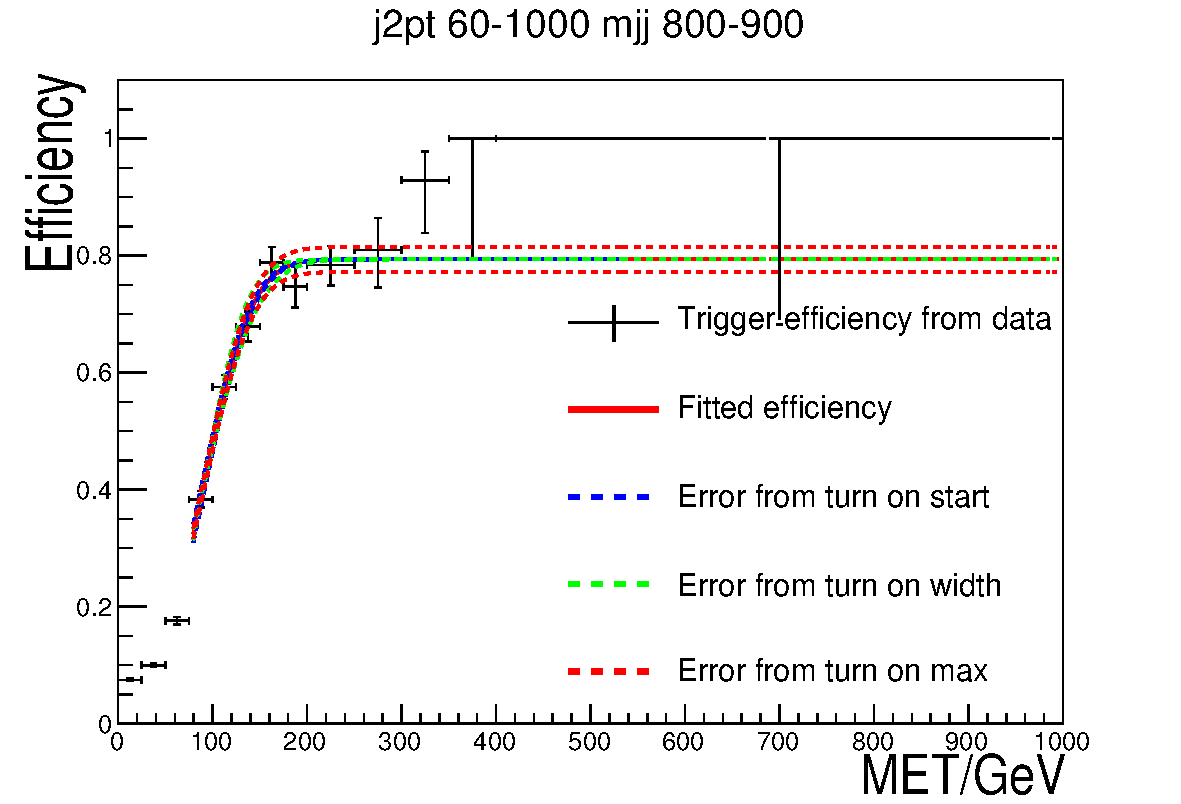
\includegraphics[width=.6\largefigwidth]{plots/parked/trigfitplots/hData_MET_1D_43BC.pdf}

    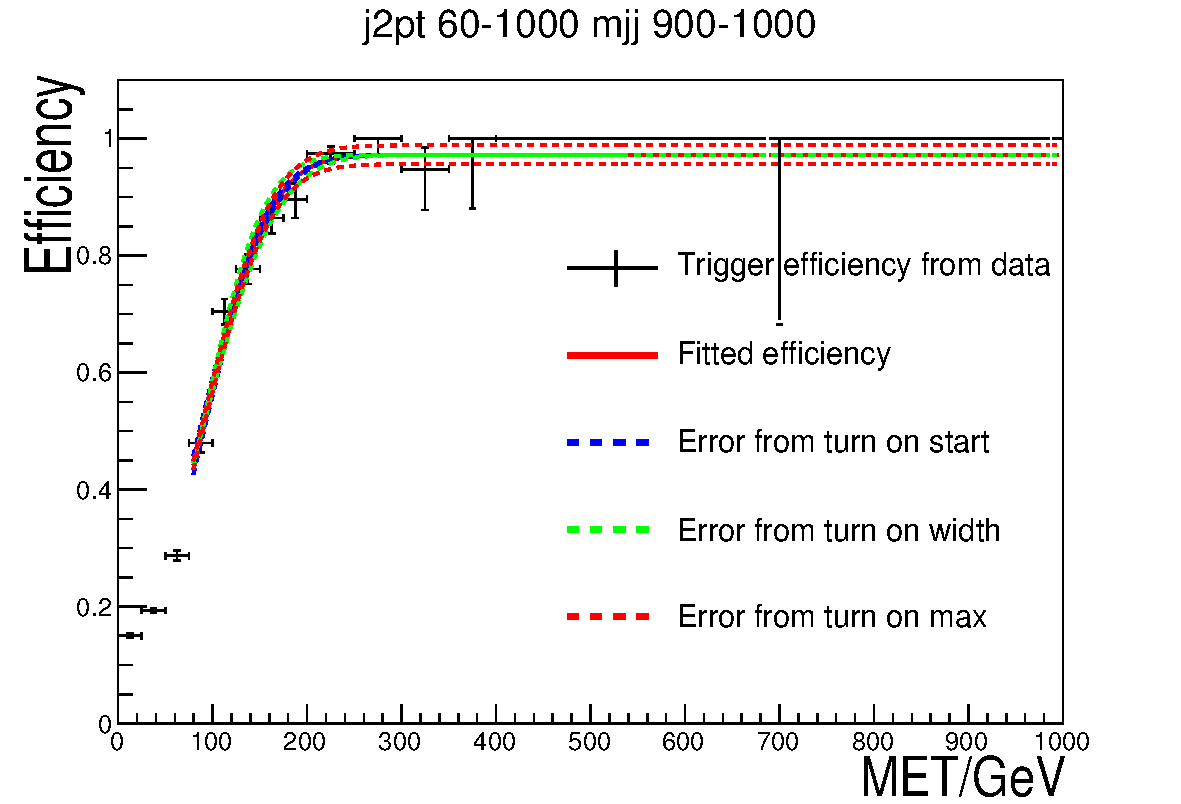
\includegraphics[width=.6\largefigwidth]{plots/parked/trigfitplots/hData_MET_1D_44BC.pdf}
    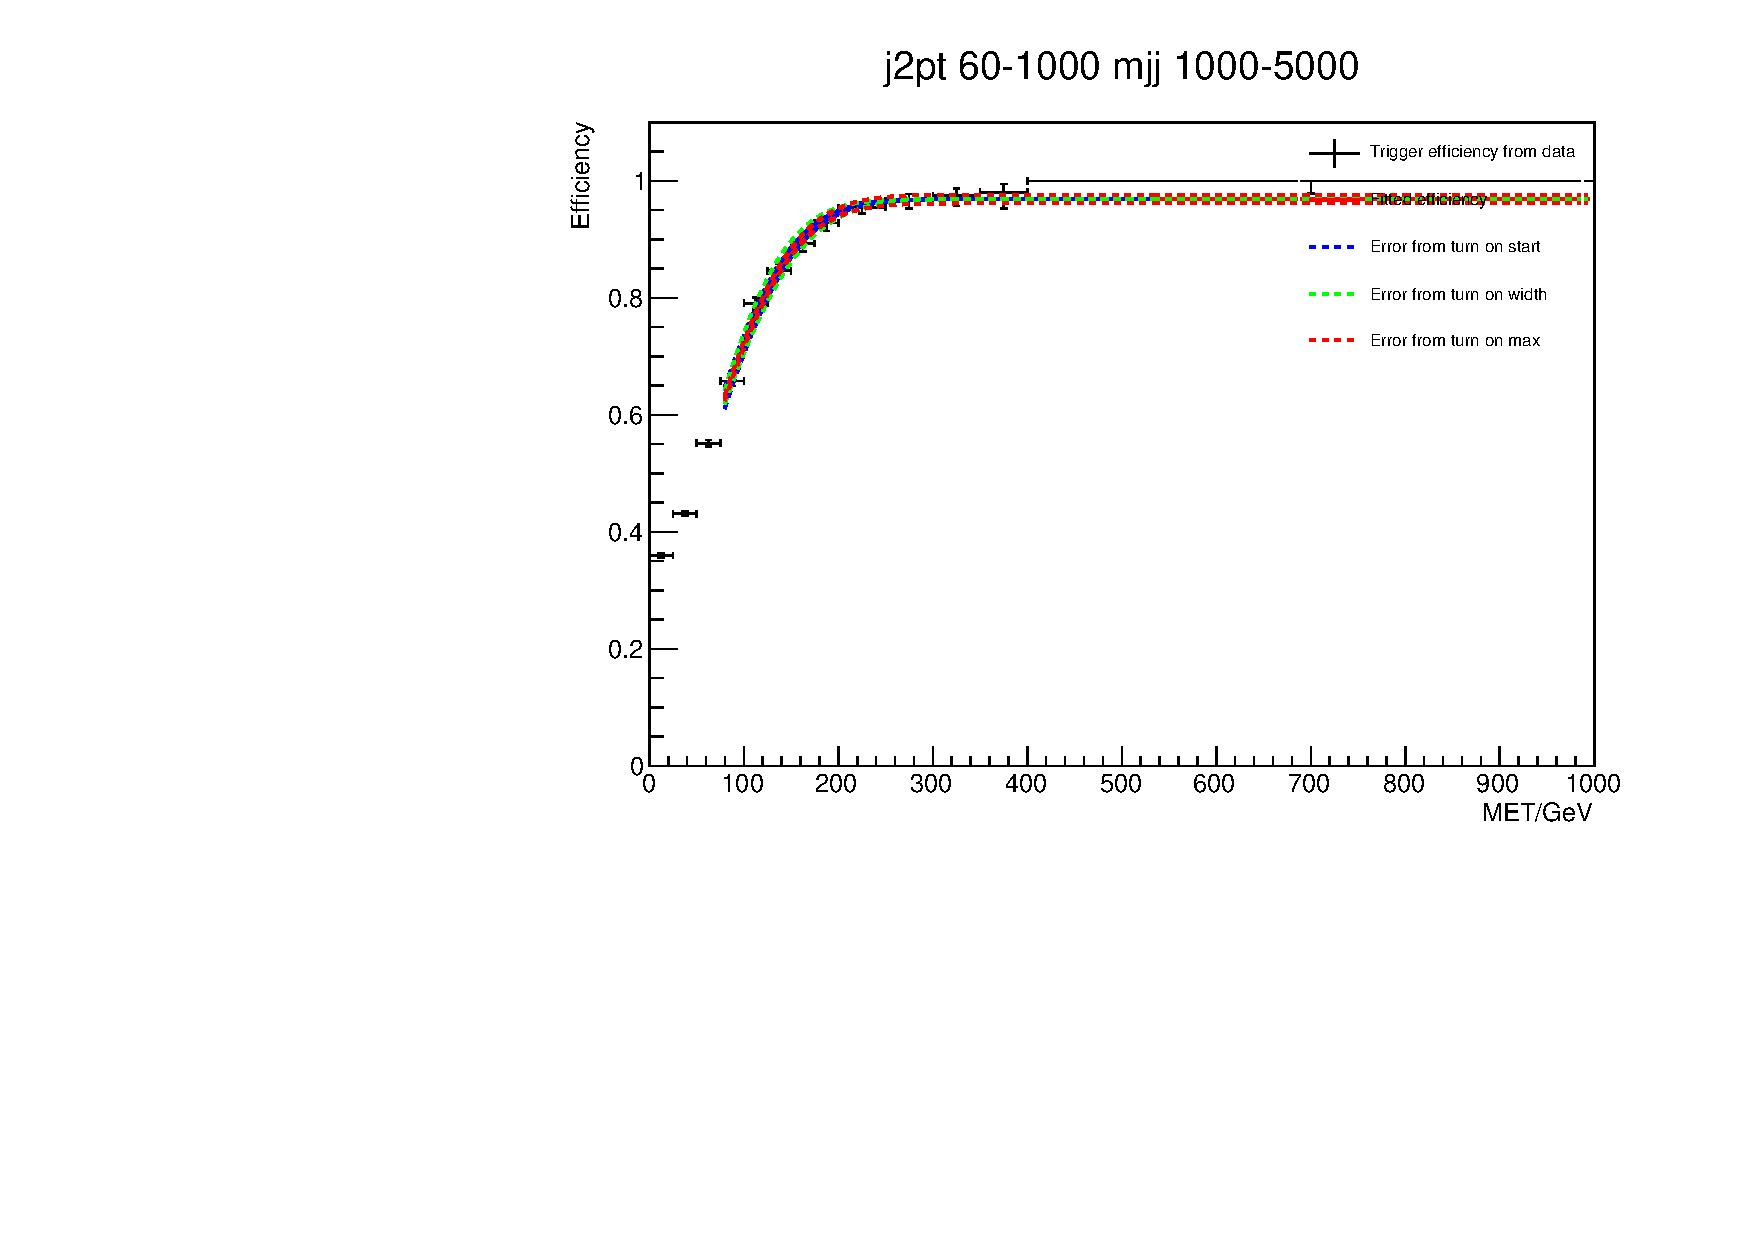
\includegraphics[width=.6\largefigwidth]{plots/parked/trigfitplots/hData_MET_1D_45BC.pdf}
    \caption{The measured efficiency of the trigger used in runs B and C as a function of MET in bins of dijet mass (mjj) and sub-leading jet $p_{T}$ (j2pt). The bin that each plot corresponds to is displayed at the top of the plot}
    \label{fig:trigfitplotsBC2}
  \end{center}
\end{figure}

\begin{figure}[h!]
  \begin{center}
    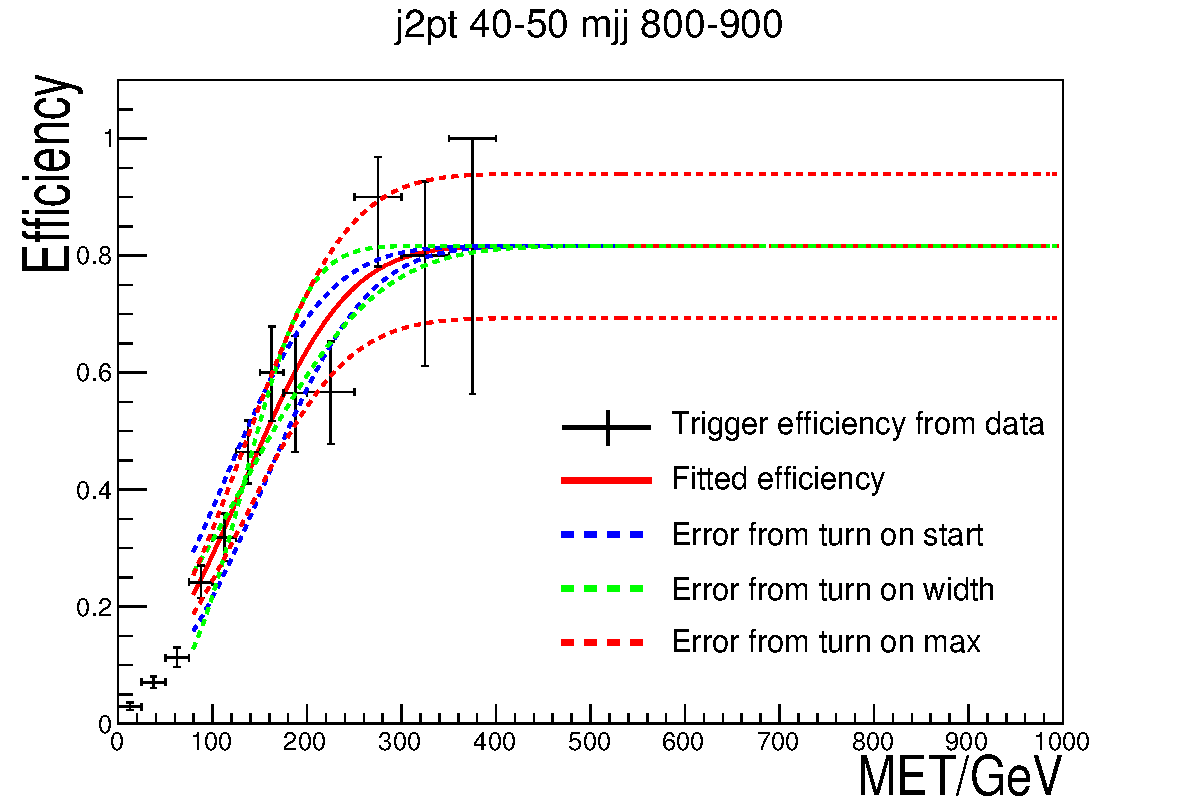
\includegraphics[width=.6\largefigwidth]{plots/parked/trigfitplots/hData_MET_1D_23D.pdf}
    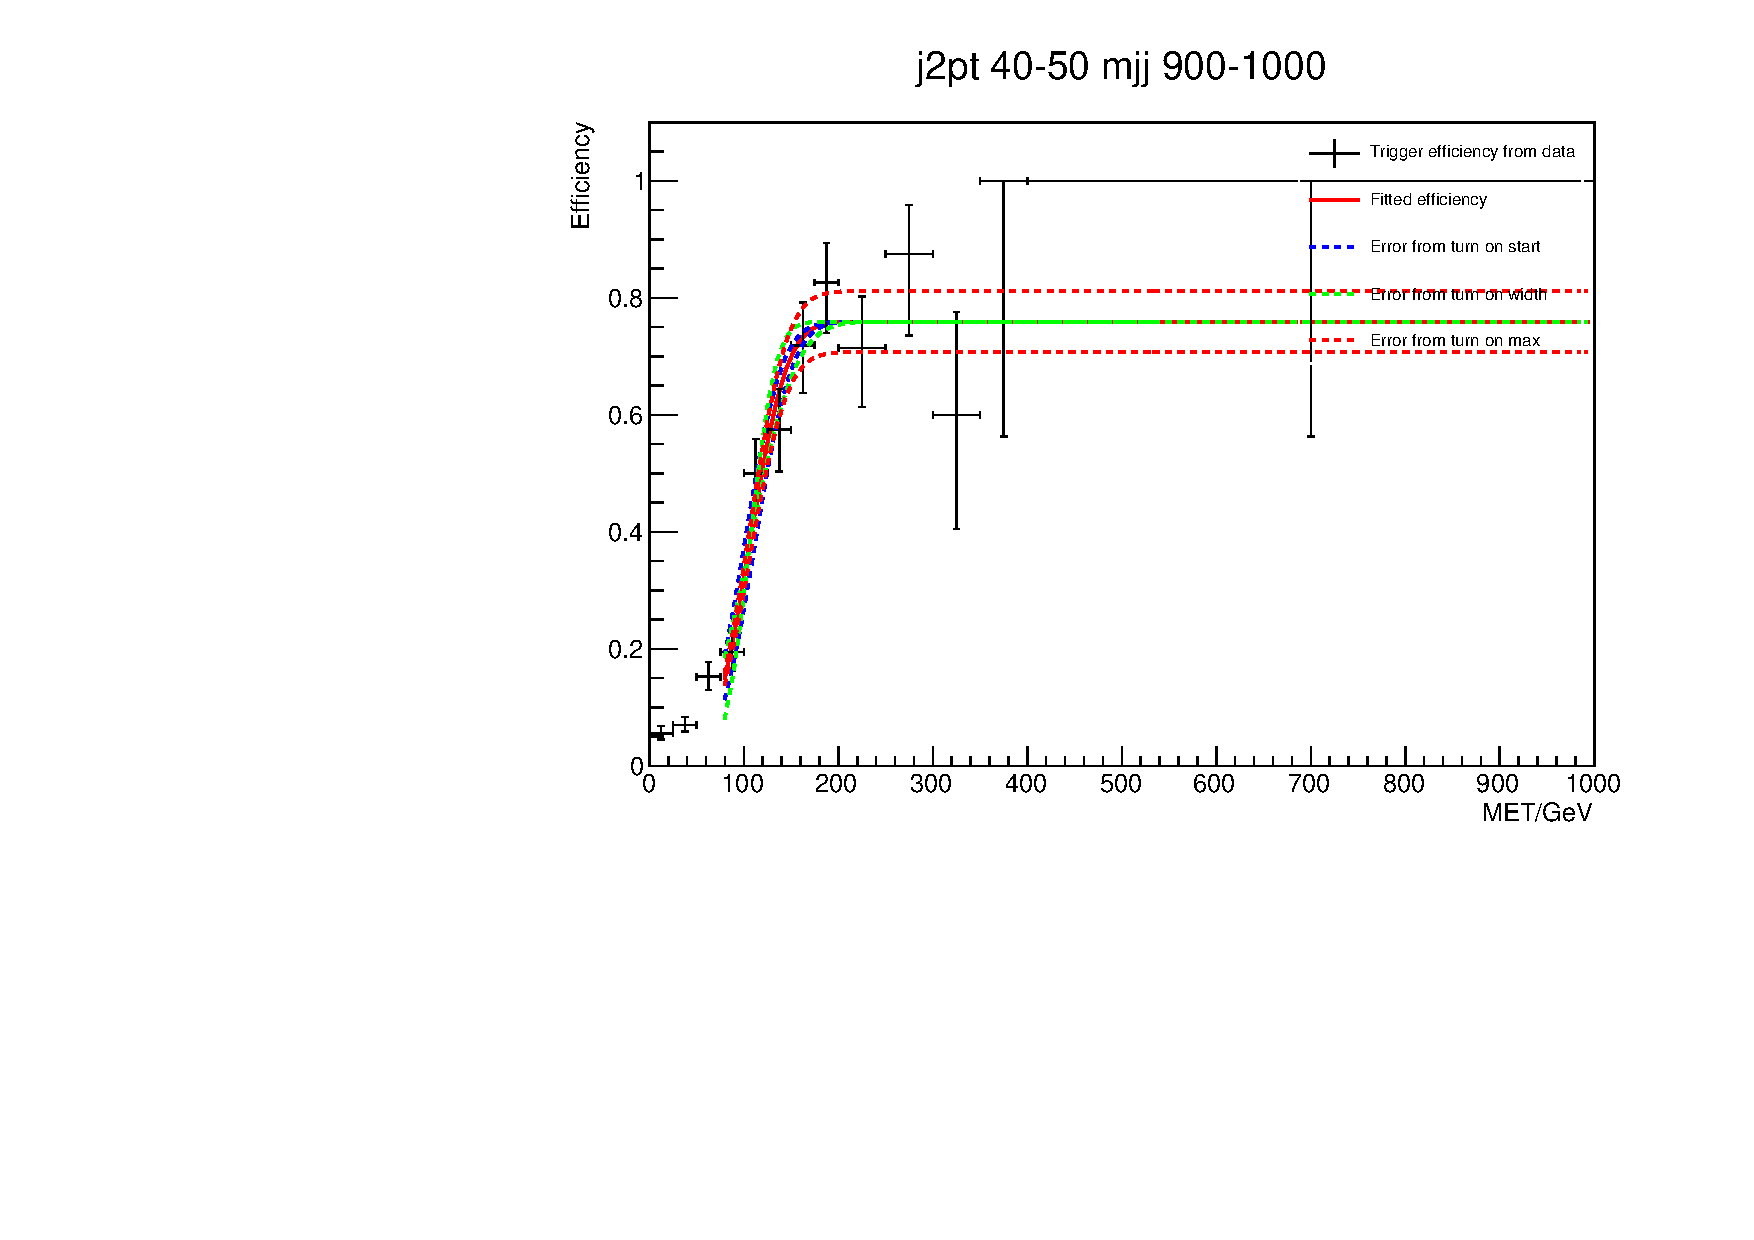
\includegraphics[width=.6\largefigwidth]{plots/parked/trigfitplots/hData_MET_1D_24D.pdf}

    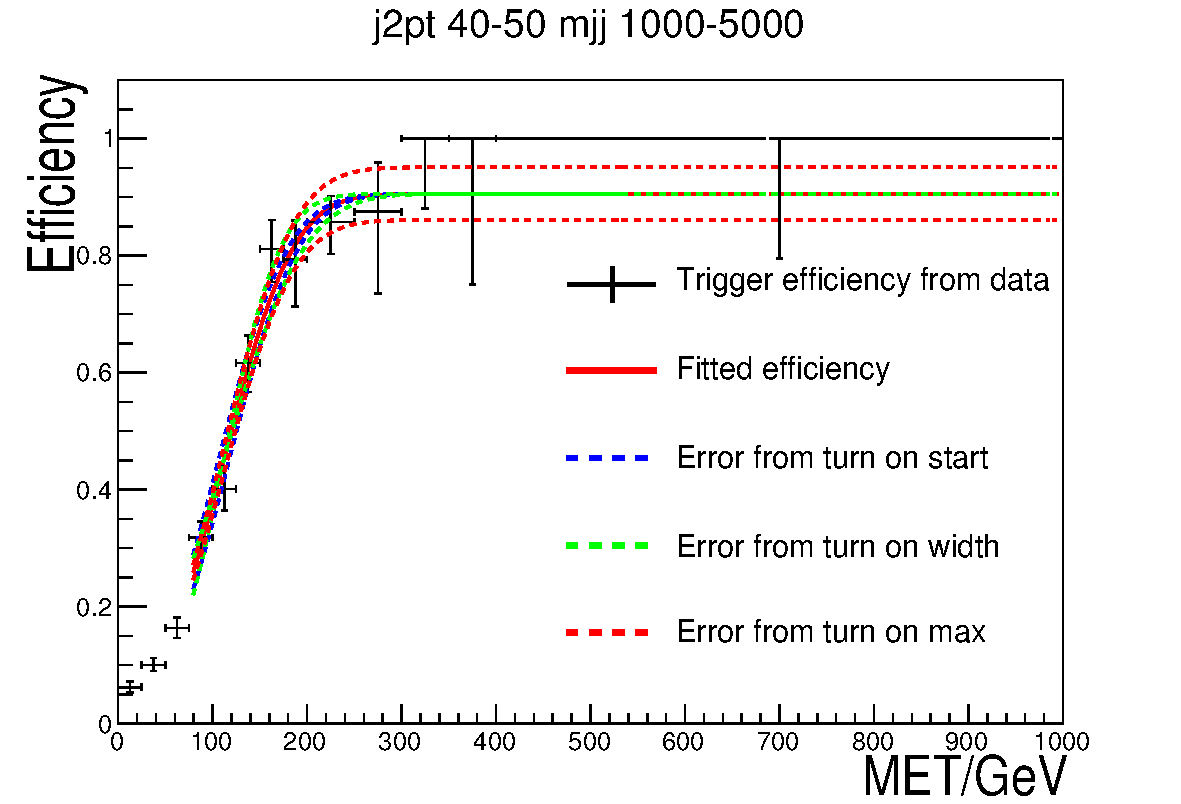
\includegraphics[width=.6\largefigwidth]{plots/parked/trigfitplots/hData_MET_1D_25D.pdf}
    \caption{The measured efficiency of the trigger used in run D as a function of MET in bins of dijet mass (mjj) and sub-leading jet $p_{T}$ (j2pt). The bin that each plot corresponds to is displayed at the top of the plot}
    \label{fig:trigfitplotsD1}
  \end{center}
\end{figure}

\begin{figure}
  \begin{center}
    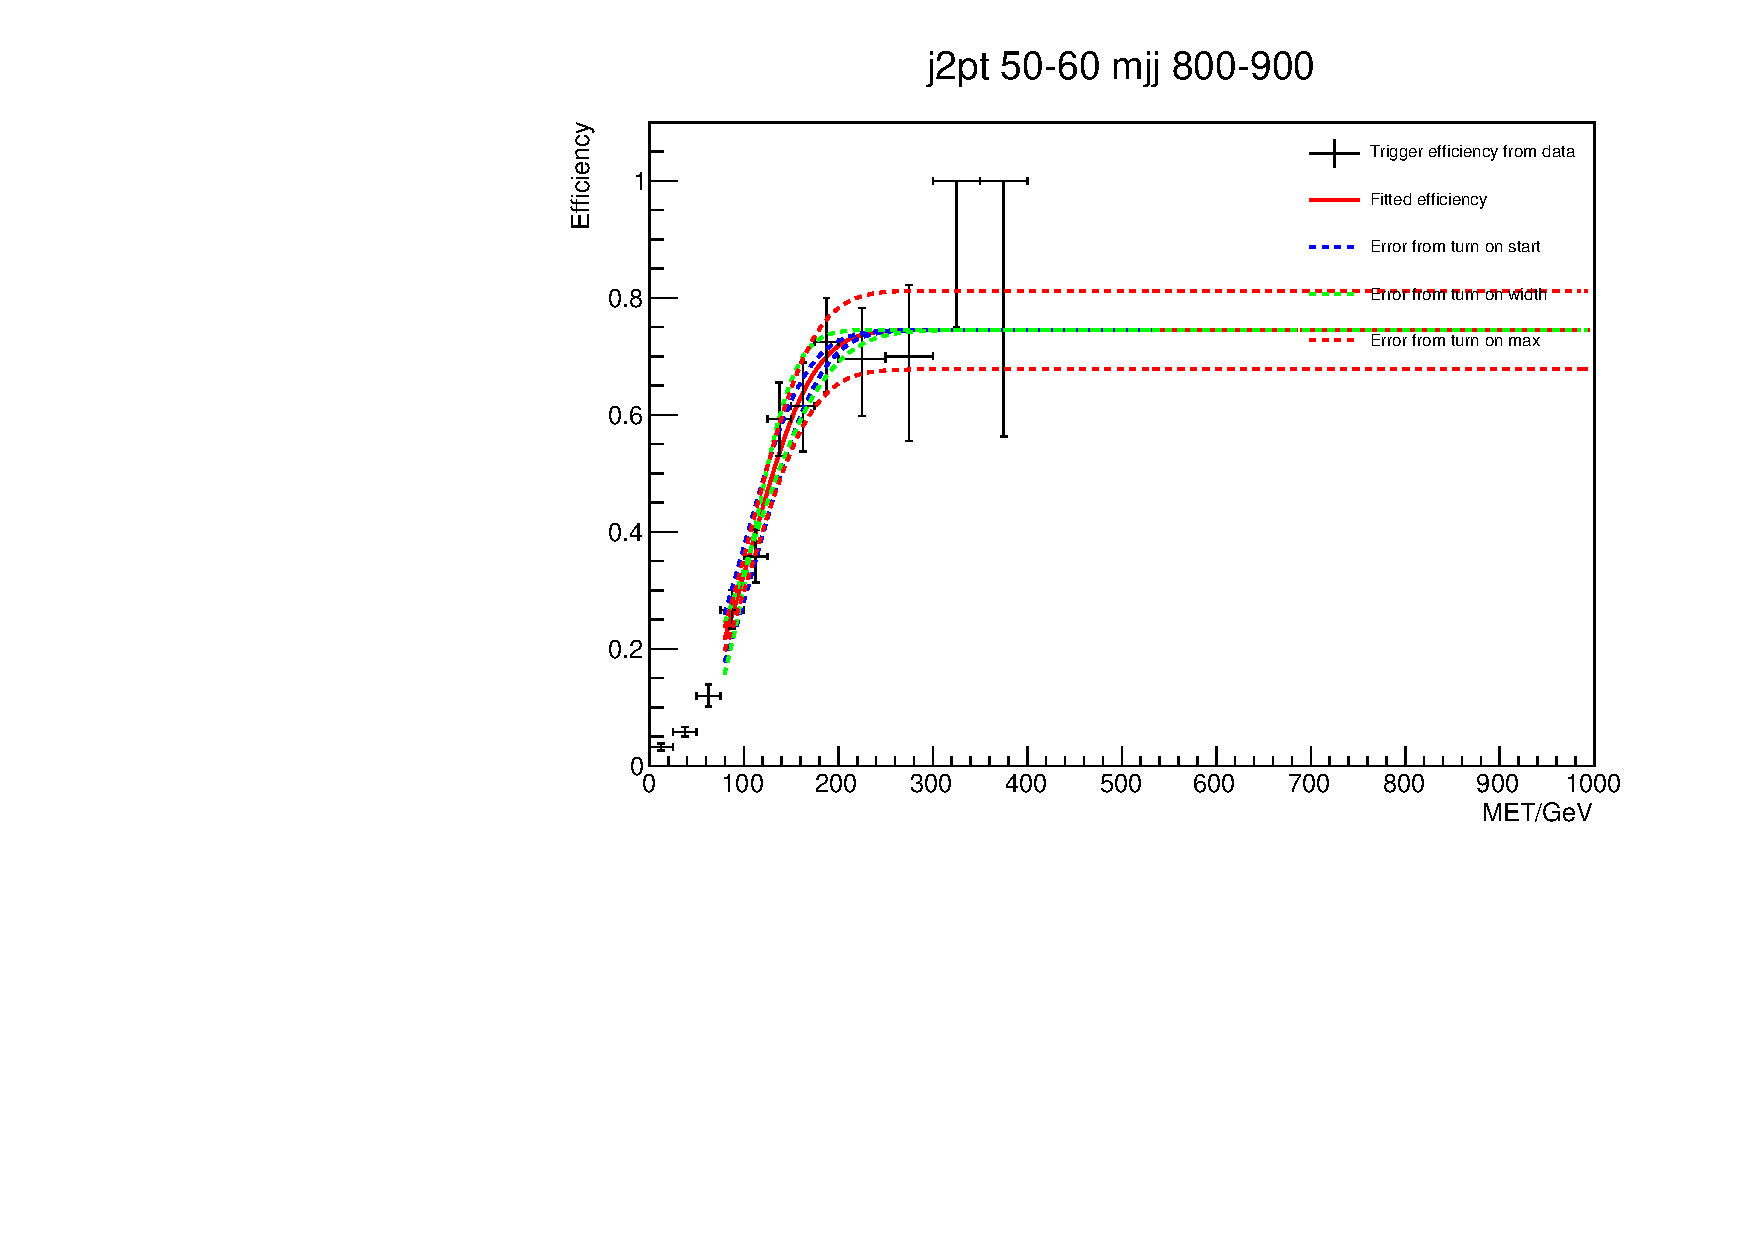
\includegraphics[width=.6\largefigwidth]{plots/parked/trigfitplots/hData_MET_1D_33D.pdf}
    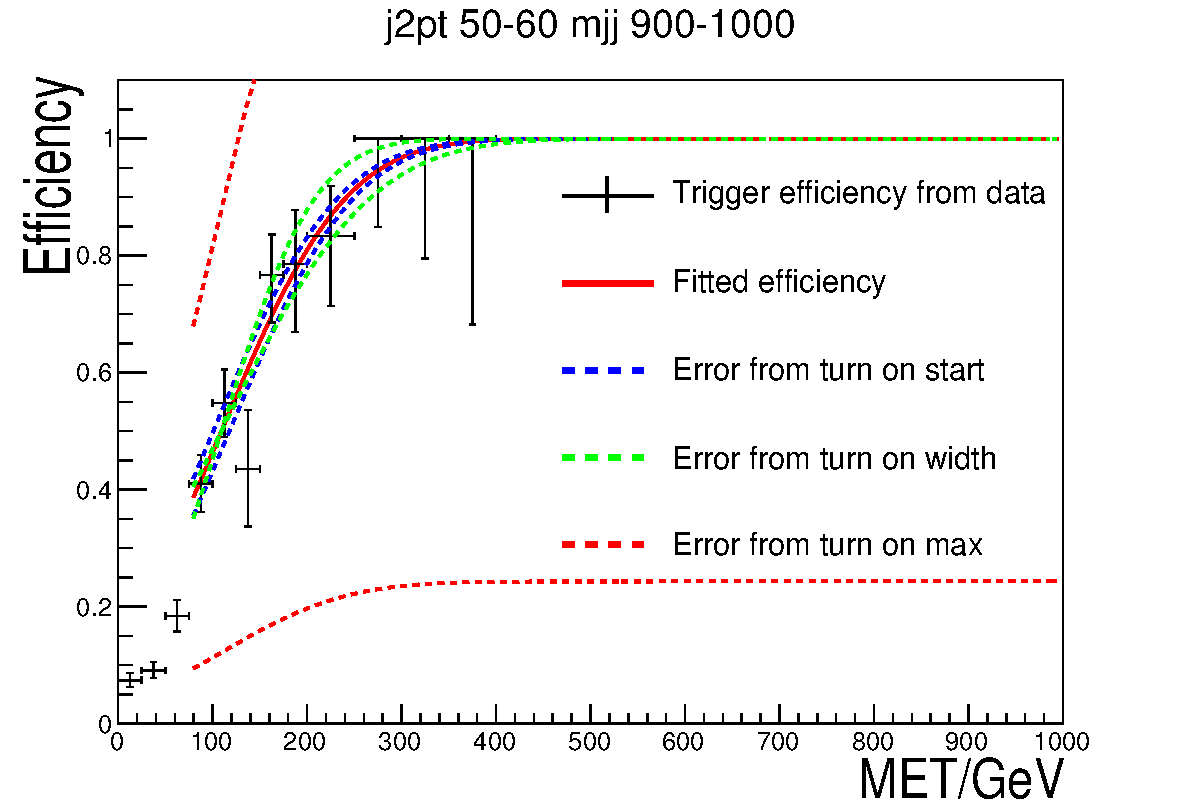
\includegraphics[width=.6\largefigwidth]{plots/parked/trigfitplots/hData_MET_1D_34D.pdf}

    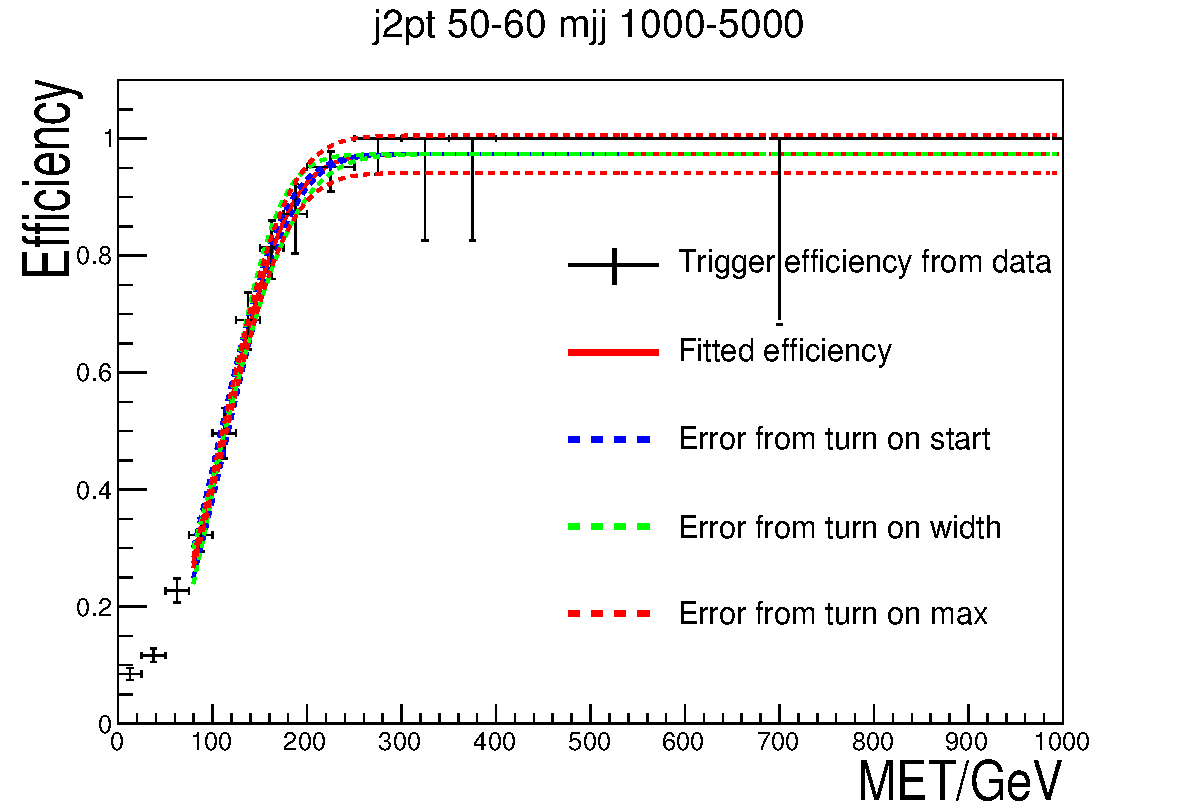
\includegraphics[width=.6\largefigwidth]{plots/parked/trigfitplots/hData_MET_1D_35D.pdf}
    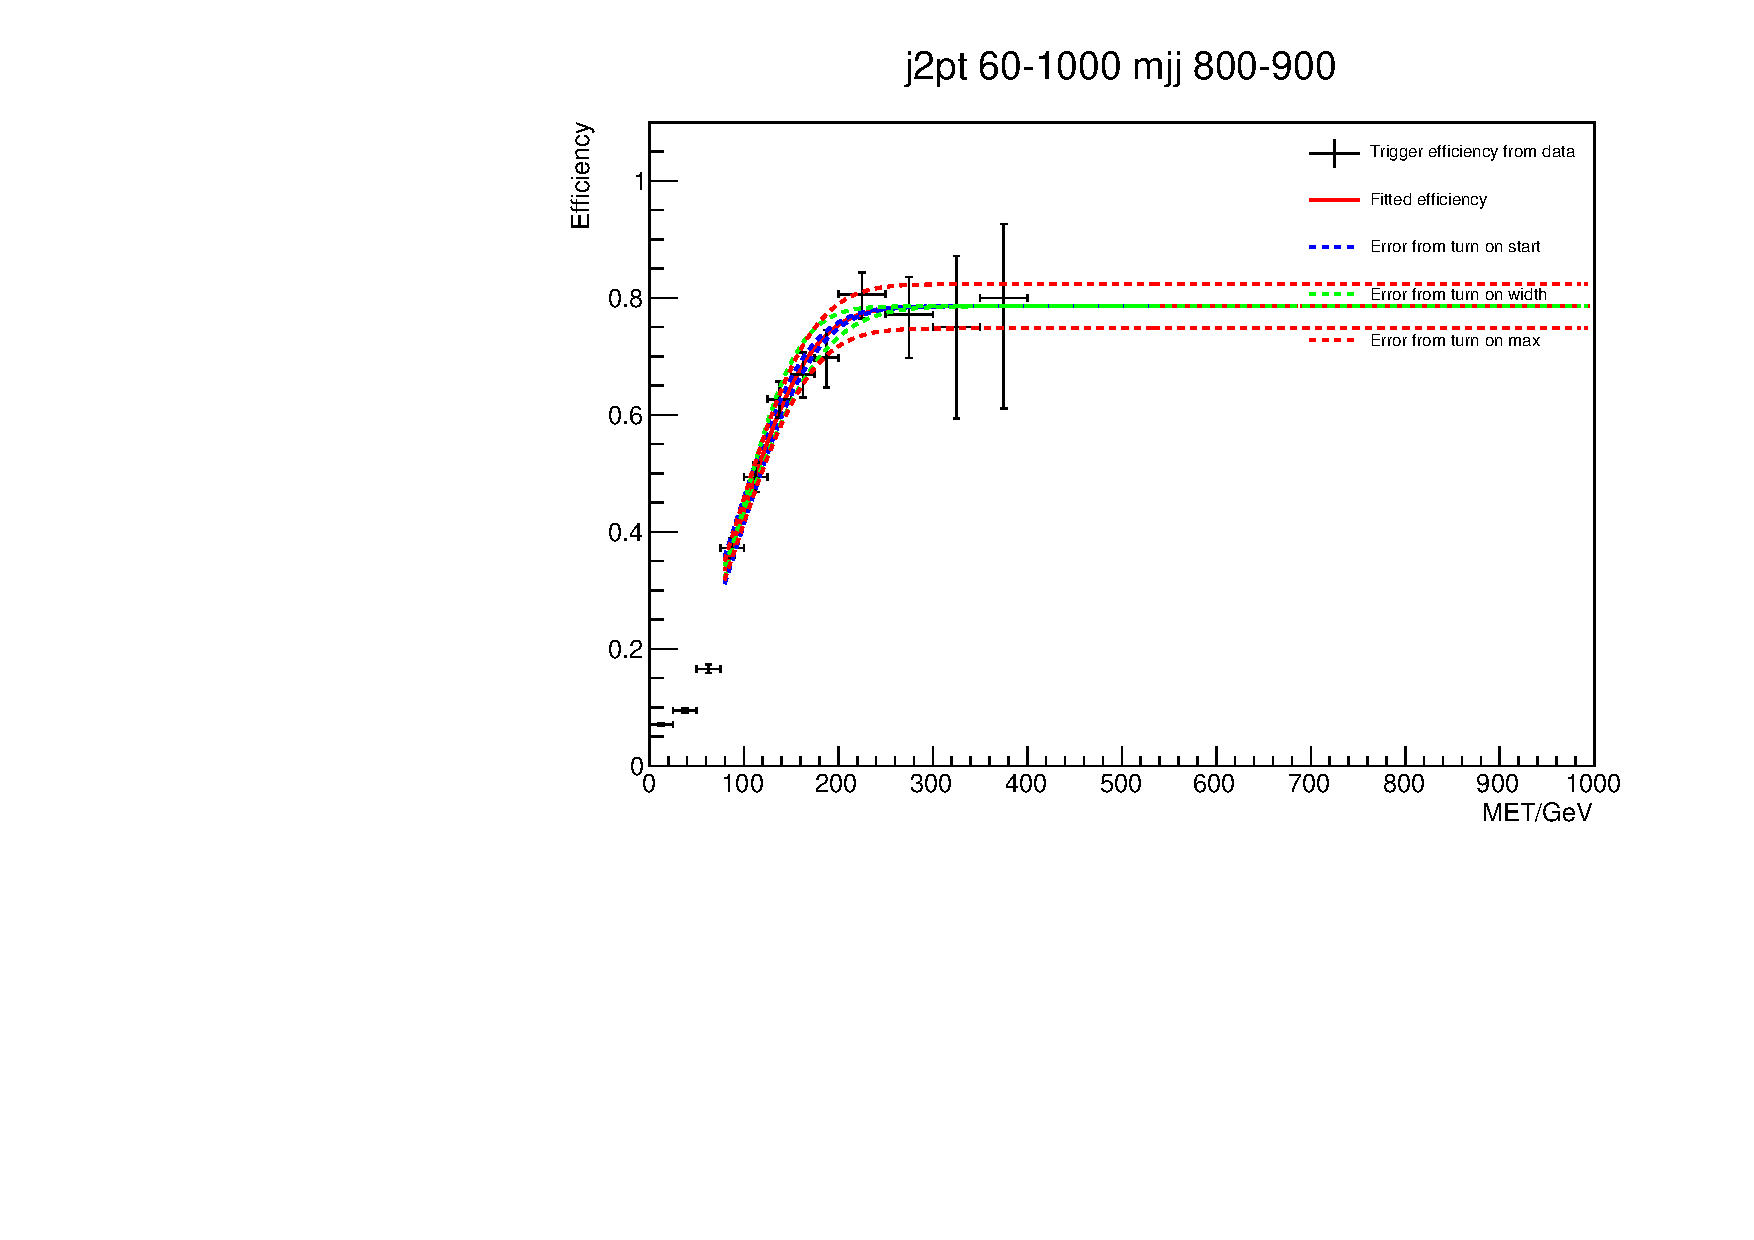
\includegraphics[width=.6\largefigwidth]{plots/parked/trigfitplots/hData_MET_1D_43D.pdf}

    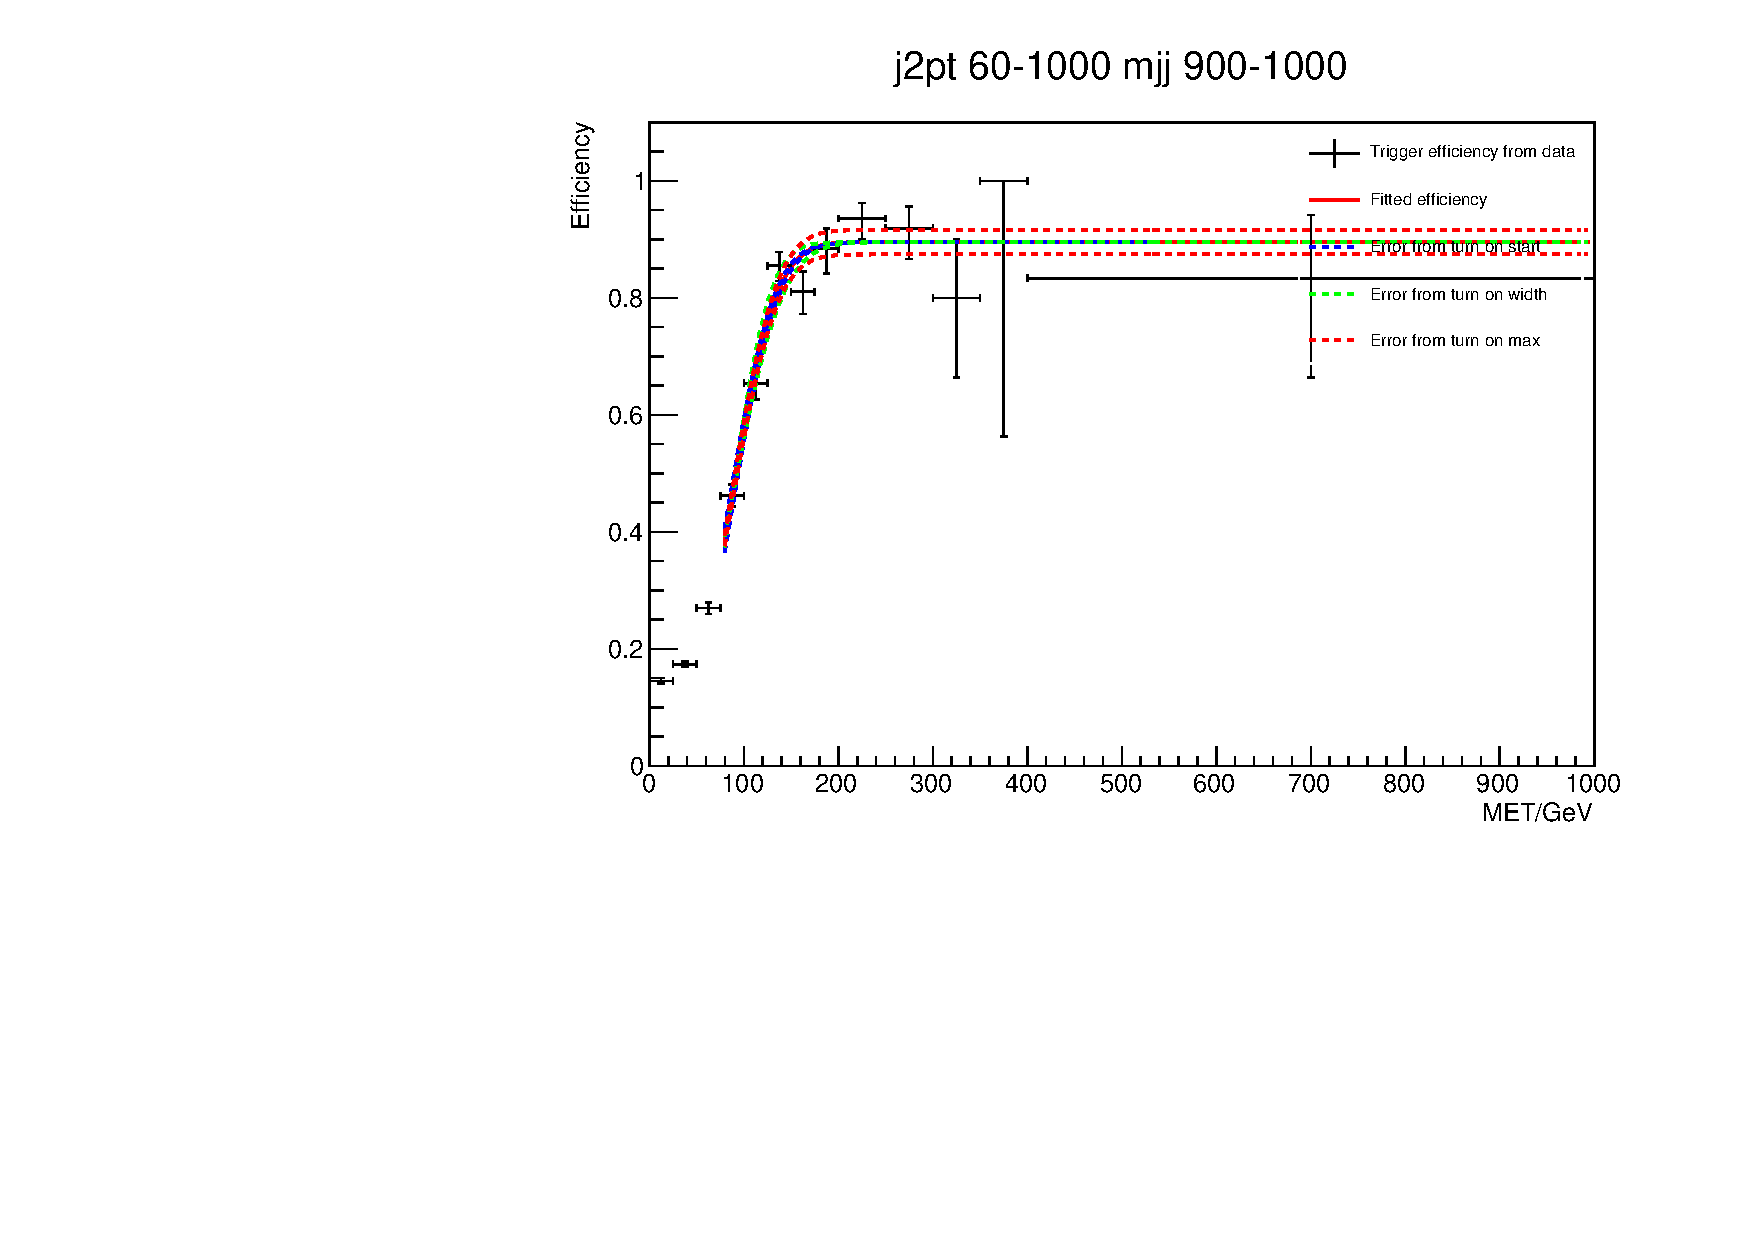
\includegraphics[width=.6\largefigwidth]{plots/parked/trigfitplots/hData_MET_1D_44D.pdf}
    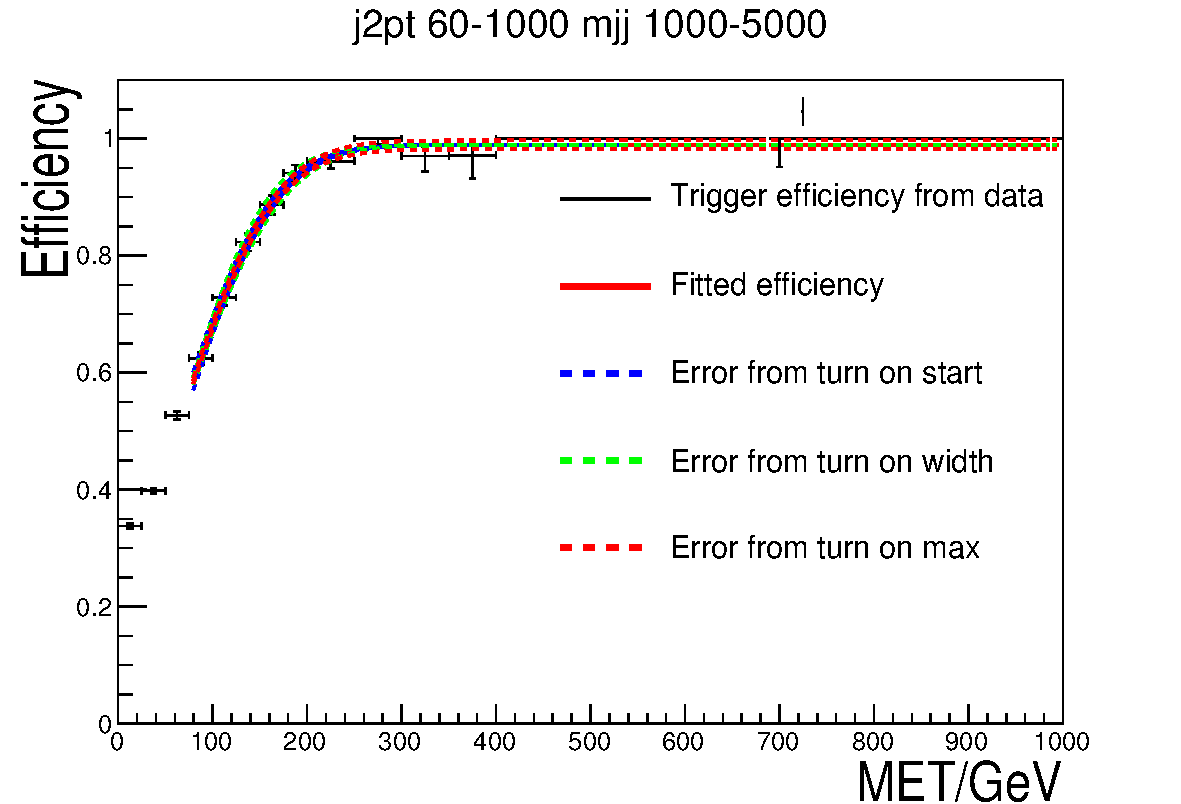
\includegraphics[width=.6\largefigwidth]{plots/parked/trigfitplots/hData_MET_1D_45D.pdf}
    \caption{The measured efficiency of the trigger used in run D as a function of MET in bins of dijet mass (mjj) and sub-leading jet $p_{T}$ (j2pt). The bin that each plot corresponds to is displayed at the top of the plot}
    \label{fig:trigfitplotsD2}
  \end{center}
\end{figure}

\end{appendices}

%% Produce the un-numbered back matter (e.g. colophon,
%% bibliography, tables of figures etc., index...)
\begin{backmatter}
  %\begin{colophon}
%  This thesis was made in \LaTeXe{} using the ``hepthesis'' class~\cite{hepthesis}.
%\end{colophon}

%!!UPDATE THIS
%% You're recommended to use the eprint-aware biblio styles which
%% can be obtained from e.g. www.arxiv.org. The file thesis.bib
%% is derived from the source using the SPIRES Bibtex service.
\bibliographystyle{lucas_unsrt}
\bibliography{thesis}
\newpage

\listoffigures
\listoftables

\chapter*{List of Acronyms}
\addcontentsline{toc}{chapter}{Acronyms}
\markboth{ACRONYMS}{}

\begin{acronym}
\vspace{0.5cm}
\acro{PSB}{Proton Synchrotron Booster}
\acro{PS}{Proton Synchrotron}
\acro{SPS}{Super Proton Synchrotron}
\acro{PU}{pile-up}
\acro{SM}{standard model}
\acro{BSM}{beyond the SM}
\acro{QFT}{quantum field theory}
\acro{ECAL}{electromagnetic calorimeter}
\acro{HCAL}{hadron calorimeter}


\acro{4FS}{four-flavour scheme}
\acro{5FS}{five-flavour scheme}
\acro{BDT}{boosted decision tree}
\acro{CL}{confidence level}
\acro{CSC}{cathode strip chamber}
\acro{CSV}{combined secondary vertex}
\acro{CTF}{combinatorial track finder}
\acro{DA}{deterministic annealing}
\acro{DAQ}{data acquisition}
\acro{DT}{drift tube}
\acro{GSF}{Gaussian sum filter}
\acro{HB}{hadron barrel}
\acro{HE}{hadron endcaps}
\acro{HF}{hadron forward}
\acro{HLT}{high-level trigger}
\acro{HO}{hadron outer}
\acro{HPS}{hadron plus strips}
\acro{JER}{jet energy resolution}
\acro{JES}{jet energy scale}
\acro{L1}{Level-1}
\acro{LHCHXSWG}{LHC Higgs Cross Section Working Group}
\acro{LO}{leading order}
\acro{MC}{Monte Carlo}
\acro{MPF}{missing transverse energy projection fraction}
\acro{MPI}{multi-parton interaction}
\acro{MVA}{multi-variate analysis}
\acro{MSSM}{minimal supersymmetric standard model}
\acro{NLO}{next-to-leading order}
\acro{NNLO}{next-to-next-to-leading order}
\acro{NNLL}{next-to-next-to-leading logarithmic}
\acro{pdf}{probability density function}
\acro{PDF}{parton distribution function}
\acro{PF}{particle flow}
\acro{PV}{Primary Vertex}
\acro{QCD}{Quantum Chromodynamics}
\acro{RF}{radio frequency}
\acro{RPC}{resistive plate chamber}
\acro{SSV}{simple secondary vertex}
\acro{TEC}{tracker endcaps}
\acro{TIB}{tracker inner barrel}
\acro{TID}{tracker inner disks}
\acro{TOB}{tracker outer barrel}
\acro{UE}{underlying event}
\acro{VBF}{vector boson fusion}
\acro{WLCG}{Worldwide LHC Computing Grid}
\end{acronym}

%% I prefer to put these tables here rather than making the
%% front matter seemingly interminable. No-one cares, anyway!

%% If you have time and interest to generate a (decent) index,
%% then you've clearly spent more time on the write-up than the 
%% research ;-)
%\printindex

\end{backmatter}

%% Close
\end{document}
